\documentclass{article}
\usepackage[utf8]{inputenc}
\usepackage[T1]{fontenc}
\usepackage{lmodern}
\usepackage[frenchb]{babel}
\usepackage{graphicx}
\usepackage[left=2cm,right=2cm,top=2cm,bottom=2cm]{geometry}
\usepackage{subcaption}
\usepackage{morefloats}

\title{Traitement des données Audio-Visuelle\\Projet}
\author{Victor Drouin Viallard}

\begin{document}

\maketitle
\clearpage
\tableofcontents
\clearpage

\section{TP 1 - Espaces de représentation des couleurs}
\paragraph{}
Le but de ce TP est d'étudier les différentes façon de représenter les images couleurs, de les projeter dans des bases adaptées, et de les réduire à des espaces plus restreints.
\subsection{Exercice 1 - Corrélations et contrastes}
\paragraph{Corrélation des espaces RVB}
Ce premier exercice propose, sur une image particulière donnée, d'observer les corrélations existantes entre les différentes composantes colorimétriques. En effet, après calcul on obtient les coefficients de corrélation suivants entre les différentes couleurs~:
\begin{itemize}
    \item Rouge/Vert~: 0.9861
    \item Rouge/Bleu~: 0.9690
    \item Vert/Bleu~: 0.9918
\end{itemize}
Ce qui montre une très force corrélation entre les couleurs, tout particulièrement entre le vert et le bleu.

\paragraph{Non corrélation locale}
En outre, comme le suggère le sujet, on observe la disparition de l'arbre central de l'image sur sa composante bleu (figure~\ref{disparition_arbre}). Cela signifie que sur cette partie de l'image la corrélation entre la composante bleu et les autres composantes est assez faible.
\begin{figure}[!ht]
    \centering
    \begin{subfigure}[c]{0.45\linewidth}
        \centering
        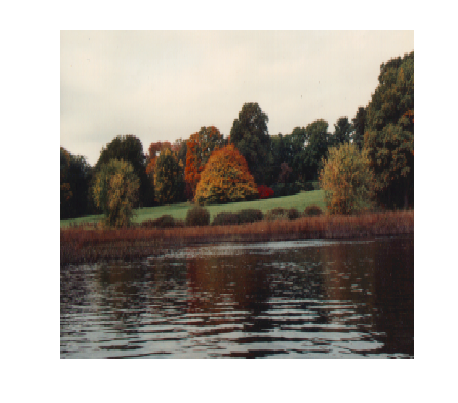
\includegraphics[width=\linewidth]{images/1-autumn_rgb.png}
        \subcaption{Image originale}
    \end{subfigure}
    \hfill
    \begin{subfigure}[c]{0.45\linewidth}
        \centering
        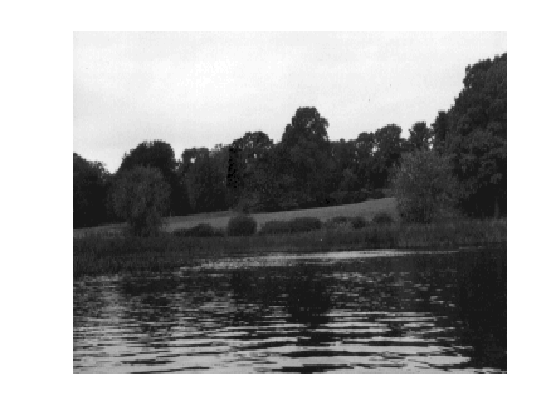
\includegraphics[width=\linewidth]{images/1-autumn_b.png}
        \subcaption{Composante bleu}
    \end{subfigure}
    \caption{Disparition de l'arbre sur la composante bleu}
    \label{disparition_arbre}
    \label{truc}
\end{figure}
Si on choisit de calculer la corrélation entre les trois canaux dans cette zone de l'image, on observe en effet des valeurs différentes de celles précédentes car la corrélation entre le rouge et le bleu diminue fortement :
\begin{itemize}
    \item Rouge/Vert~: 0.8079
    \item Rouge/Bleu~: 0.1979
    \item Vert/Bleu~: 0.6671
\end{itemize}

d'où la disparition.

\paragraph{Contraste}
Le calcul de la variance des différentes composantes puis du contraste de l'image permet d'observer son faible niveau. Il est de : 0.3795 et se répartit comme suit entre les couleurs :
\begin{itemize}
    \item Rouge~: 0.3358
    \item Vert~: 0.3462
    \item Bleu~: 0.3179
\end{itemize}
Cette répartition uniforme est attendue du fait de la corrélation fortes entre les couleurs.

\paragraph{Transformation d'une image couleur en image noir et blanc}
Pour finir l'appel du script \emph{exercice\_2.m} sur l'image \emph{gantrycrane.png} permet, comme le laisse entendre le sujet, d'observer pourquoi le procédé de transformation d'une image couleur en image noir et blanc ne peut se faire par simple réduction à un canal choisi arbitrairement (figure~\ref{transmission_canal_bleu}). En effet, une image dont le contraste est, par exemple, dû à sa composante rouge ne pourra être transformée en noir et blanc en ne conservant que sa composante bleu sans quoi elle paraîtrait unie.
\begin{figure}[!ht]
    \begin{center}
        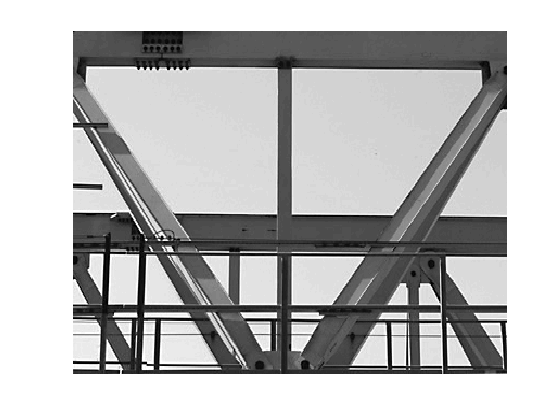
\includegraphics[width=0.6\linewidth]{images/1-gantrycrane_b.png}
        \caption{Transformation en noir et blanc par conservation du canal bleu}
        \label{transmission_canal_bleu}
    \end{center}
\end{figure}

\subsection{Exercice 2 - Analyse en composantes principales}
\paragraph{ACP}
Pour faire face au problème ennoncé plus haut qui est celui de la réduction d'un jeu de données par projection dans un espace de dimmension inférieur, l'idée la plus intéressante consiste à effectuer une analyse en composantes principales de l'objet. Celle-ci revient à trouver une base orthonormée de l'espace de départ pour laquelle la première composante représente la direction de plus grande variance, etc. En effectuant cette ACP sur la seconde image on observe la répartition des coefficiants selon les trois composantes (figure~\ref{acp_gantrycrane}).
\begin{figure}[!ht]
    \centering
    \begin{subfigure}[c]{0.32\linewidth}
        \centering
        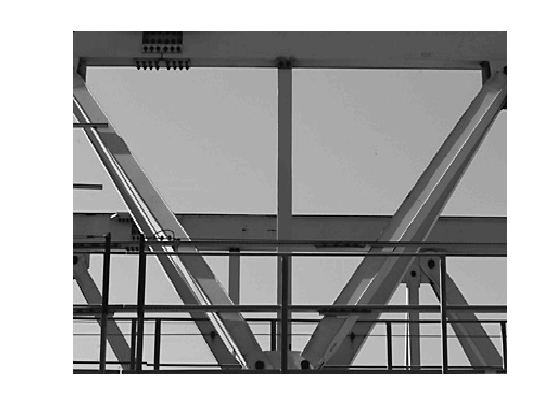
\includegraphics[width=\linewidth]{images/1-gantrycrane_c1.png}
    \end{subfigure}
    \hfill
    \begin{subfigure}[c]{0.32\linewidth}
        \centering
        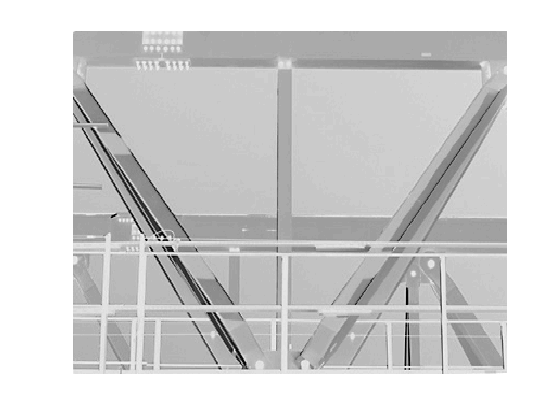
\includegraphics[width=\linewidth]{images/1-gantrycrane_c2.png}
    \end{subfigure}
    \hfill
    \begin{subfigure}[c]{0.32\linewidth}
        \centering
        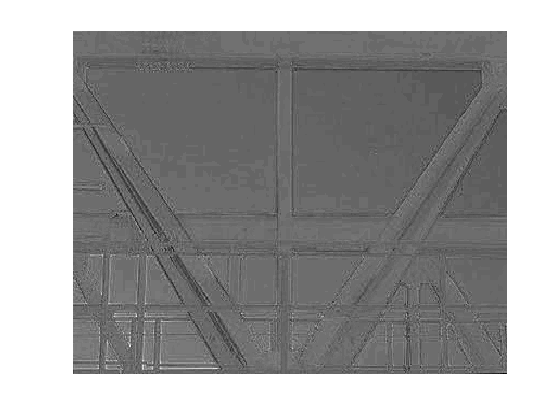
\includegraphics[width=\linewidth]{images/1-gantrycrane_c3.png}
    \end{subfigure}
    \caption{Résultat de l'analyse en composantes principales}
    \label{acp_gantrycrane}
\end{figure}
On voit alors que la première composante principale contient une information très proche de celle de l'image originale : c'est celle-ci qu'il faudrait transmettre pour une télévision en noir est blanc.
\paragraph{Conservation du constraste}
Pour la première image on réalise la même opération pour s'appercevoir alors que le la proportion de contraste est presque intégralement dûe à la première composante :
\begin{itemize}
    \item c1~: 0.9883
    \item c2~: 0.0103
    \item c3~: 0.0013
\end{itemize}
Cela est bien évidemment dû à la très forte corrélation entre les trois canaux de couleur. Enfin on remarque que le contraste se conserve entre les deux décompositions : cela est bien sûr le cas car le calcum du contraste est général au jeu de donnée et parfaitement indépendant de la base orthonormale dans laquelle elles sont exprimées.

\subsection{Exercice 3 - Combinaison des canaux RVB}
\paragraph{L'inconvénient de l'ACP}
Cette méthode de projection pour garder un maximum de contraste est la plus efficace mais extrêment coûteuse car nécessite pour chaque image de calculer et d'inverser la matrice de variance / covariance. La méthode retenue pour transmettre une image noir et blanc depuis une image en couleur a donc été d'effectuer une combinaison linéaire des trois canaux. On peut chosir plusieurs combinaisons linéaire différentes. Le sujet nous suggère de comparer celle uniforme et celle utilisée par la méthode \emph{rgb2gray} de Matlab (figure~\ref{combinaisons_canaux}).
\begin{figure}[!ht]
    \centering
    \begin{subfigure}[c]{0.45\linewidth}
        \centering
        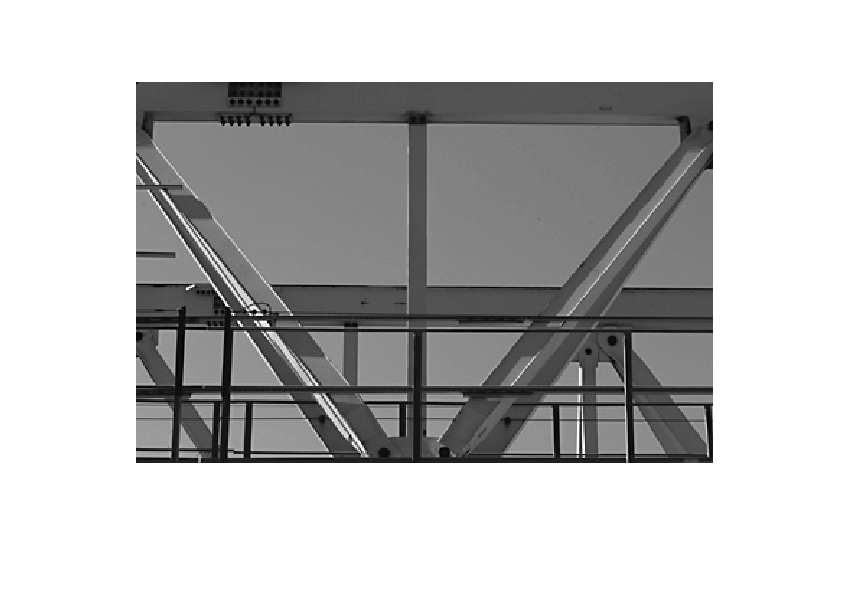
\includegraphics[width=\linewidth]{images/1-uniform.png}
        \subcaption{Combinaison uniforme}
    \end{subfigure}
    \hfill
    \begin{subfigure}[c]{0.45\linewidth}
        \centering
        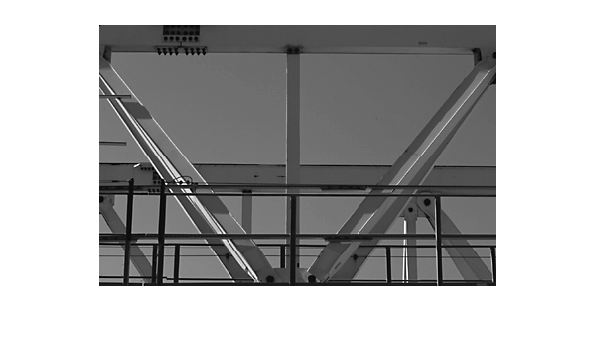
\includegraphics[width=\linewidth]{images/1-rgb2gray.png}
        \subcaption{Combinaison par \emph{rgb2gray}}
    \end{subfigure}
    \caption{Transformation en noir et blanc par combinaisons linéaires des canaux de couleur}
    \label{combinaisons_canaux}
\end{figure}
Parmi toutes ces images en noir est blanc, c'est l'image issue du canal bleu qui paraît avoir le meilleur contraste mais cela est particulier et dû au fait que :
\begin{itemize}
    \item le bleu est effectivement un facteur de contraste de l'image
    \item l'ACP produisant des valeurs de coefficient négatives, l'affichage de la composante principale est biaisé
    \item la fonction d'affichage de matlab \emph{imshow} étale le spectre de l'image affichée ce qui peut conduire à un affichage qui paraît plus contrasté dans ce cas particulier
\end{itemize}
\clearpage
\section{TP 2 - Eigenfaces}
Le but de ce TP est d'utiliser l'ACP pour établir une base de conaissance capable de restaurer une image dégradée à partir de sa projection dans cette base.
\subsection{Exercice 1 - Analyse en composantes principales}
Ce premier exercice ne présente pas de difficulté particulière mais permet de bien se rendre compte  du résultat de l'ACP sur un tel ensemble de données (figure~\ref{acp_faces}). On oberve en effet, sans doute car il y a des individus différents d'une photo à l'autre, que la première composante principale ne ressemble plus vraiment à un visage.
\begin{figure}[!ht]
    \begin{center}
        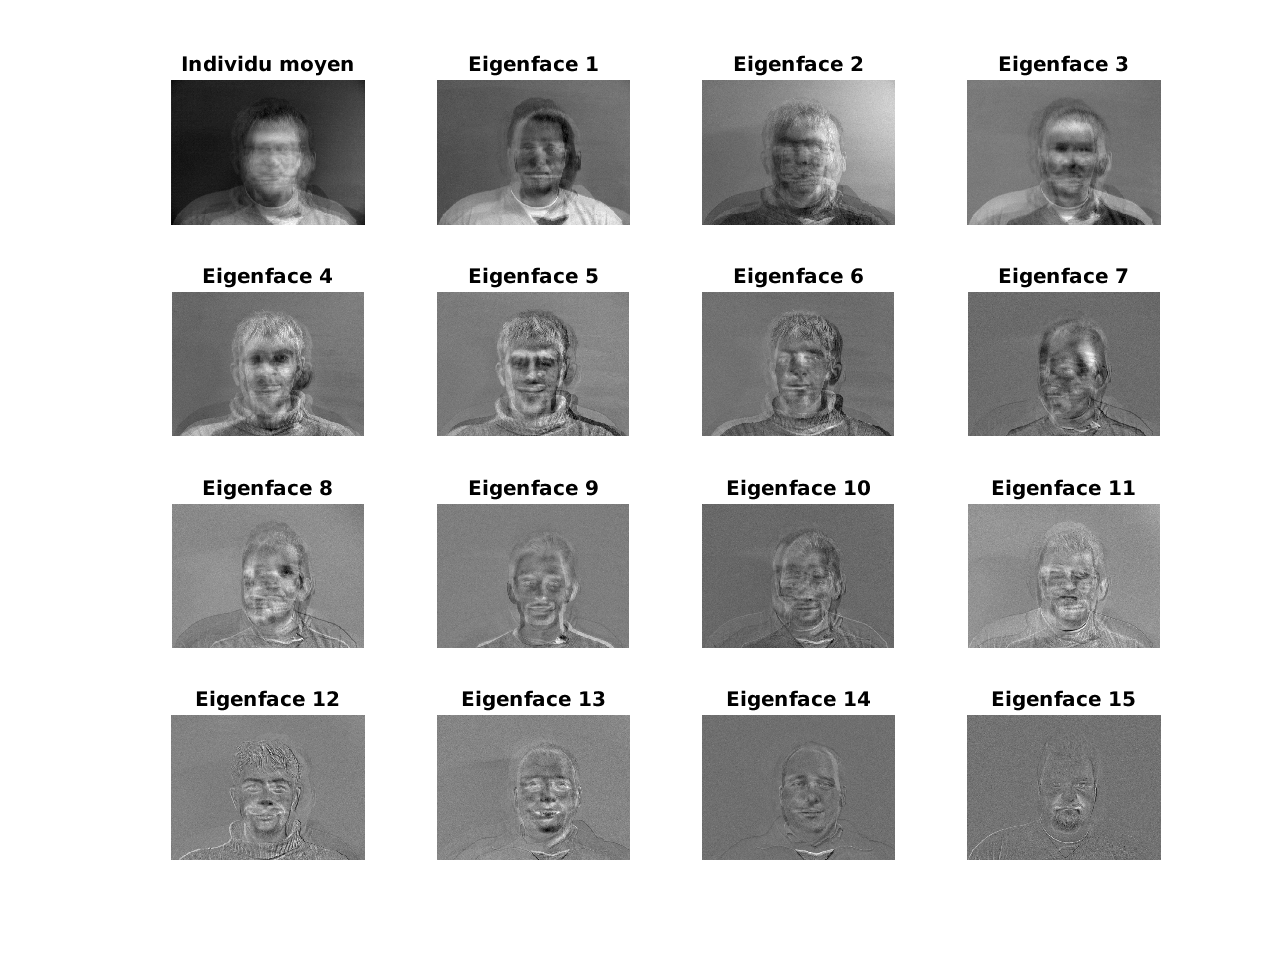
\includegraphics[width=0.9\linewidth]{images/2-acp_faces.png}
        \caption{Analyse en composantes principales des visages}
        \label{acp_faces}
    \end{center}
\end{figure}

\subsection{Exercice 2 - Projection des images sur les eigenfaces}
\paragraph{Différences selon l'individu et les images}
Dans cette exercice on nous propose d'exprimer les images des sujets dans la nouvelle base (celle composée des eigenfaces), puis de ne conserver qu'un certain nombre de composantes (projections selon les composantes de plus petit ordre) pour établir différentes "compressions" et les comparer. Par exemple en choisissant de ne conserver que 6 eigenfaces (sur 15) en plus de la valeur de l'infividu moyen, on obtient le résultat figure~\ref{proj_faces}.
\begin{figure}[!ht]
    \begin{center}
        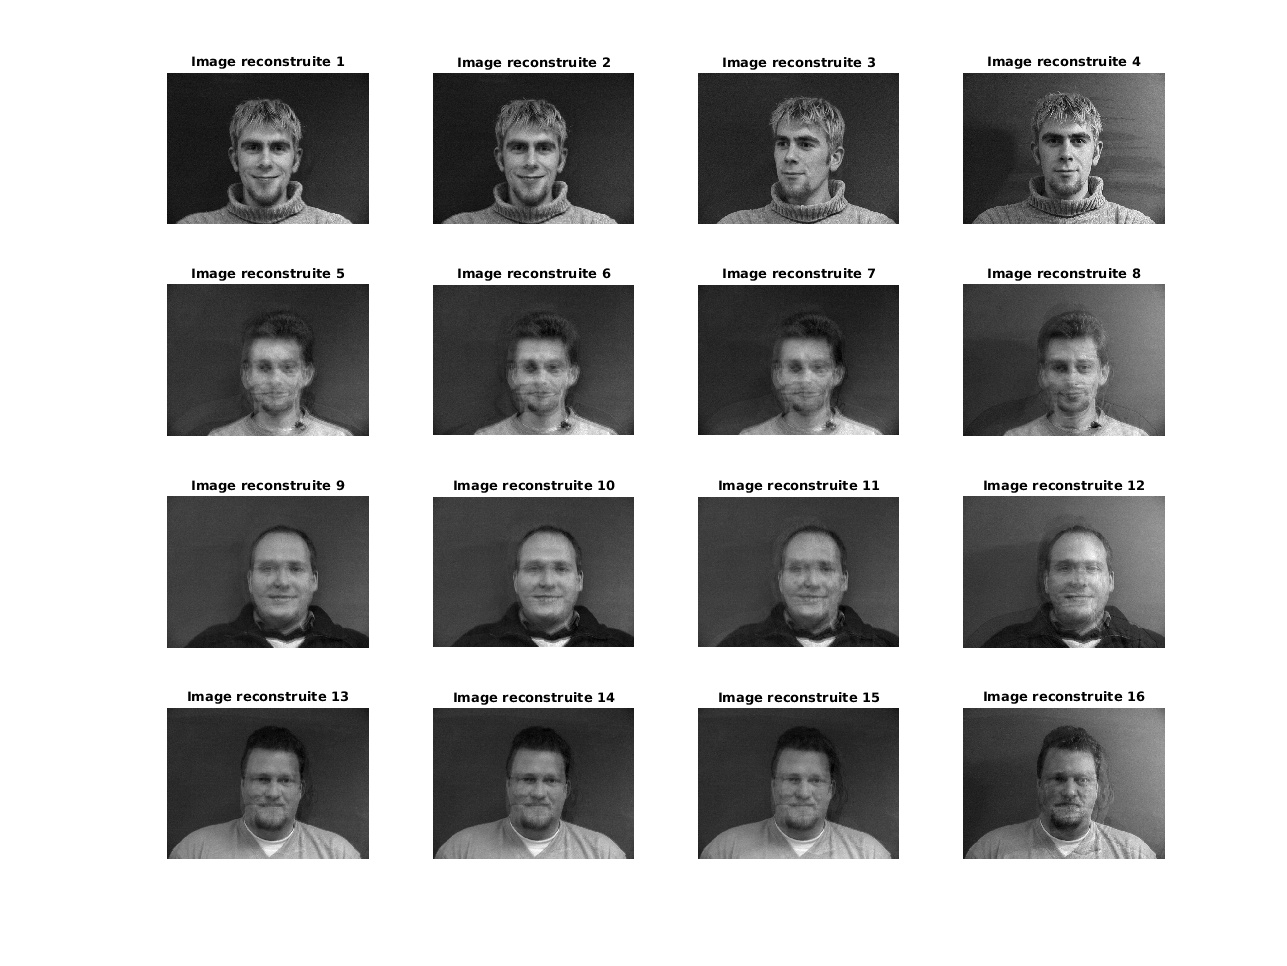
\includegraphics[width=0.9\linewidth]{images/2-proj6.png}
        \caption{Projections des visages sur un sous espace composé des 6 eigenfaces principales}
        \label{proj_faces}
    \end{center}
\end{figure}
Ici on remarque que les images ne sont toute pas aussi bien conservées. En effet celles de l'individu 1 sont bien plus ressemblantes des images originales que celles des individus 2, 3, et 4 (ces dernières sont assez floues). Cela vient certainement du fait que les images de ce premier individu sont bien plus proches de l'individu moyen que les autres (un peu comme dans de cas de l'ACP d'une image dont le contraste est principalement dû à sa composante bleu, sa composante principale sera alors proche de sa composante bleu). De plus on observe que les projections des images de l'individu 4 se ressemble beaucoup : cette fois cela doit venir du fait que les différences entre les images de cet individu sont très faibles et donc leur informations doivent être contenues selon des composantes de l'ACP d'ordre bien plus élevés (et celles-ci ne sont pas ici conservées puisqu'on s'intéresse à tous les individus en même temps).

\paragraph{Comparaison selon la dimension du sous-espace}
Par la suite on calcul la moyenne de l'écart au carré des images à leurs projections dans des espaces issus de plus ou moins d'eigenfaces pour observer la différences de "respect de l'image originale" de ces différents espaces. Comme on pouvait s'y attendre, celle-ci diminue à mesure que l'on conserve d'avantage d'eigenfaces : cela n'est pas surprenant puisqu'on conserver alors des espaces plus grands qui vont permettre de mieux distinguer les images les unes des autres (voir figure~\ref{rmse}).
\begin{figure}[!ht]
    \begin{center}
        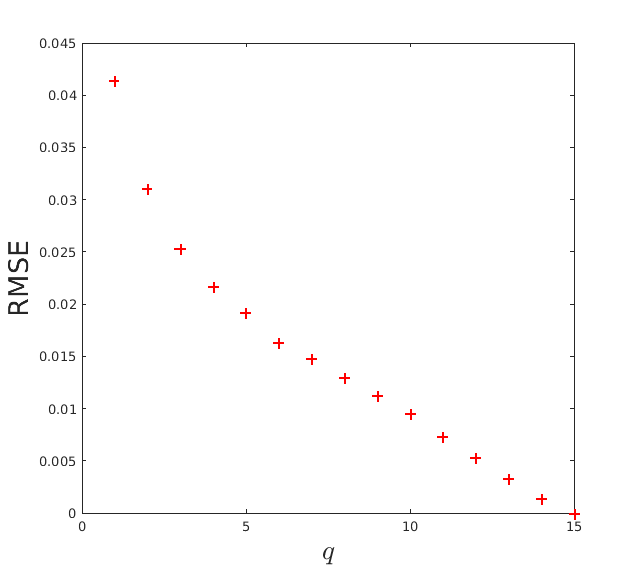
\includegraphics[width=0.6\linewidth]{images/2-rmse.png}
        \caption{RMSE en fonction du nombre de composantes principales conservées (sur 15)}
        \label{rmse}
    \end{center}
\end{figure}

\subsection{Exercice 3 - Restauration d'images dégradées}
Ici on décide de restaurer des images à partir de leur versions dégradées par une bande noire obstruant une partie plus ou moins grande de leur surface. Pour cela on projette donc l'image dégradée dans la base de issue de l'ACP puis on considère cette projection comme étant l'image non dégradée. Ainsi pour des bandes d'altération de tailles différentes on observe les résultats figure~\ref{reconstitution_bandes_noires}.
\begin{figure}[ht]
    \centering
    \begin{subfigure}[c]{0.7\linewidth}
        \centering
        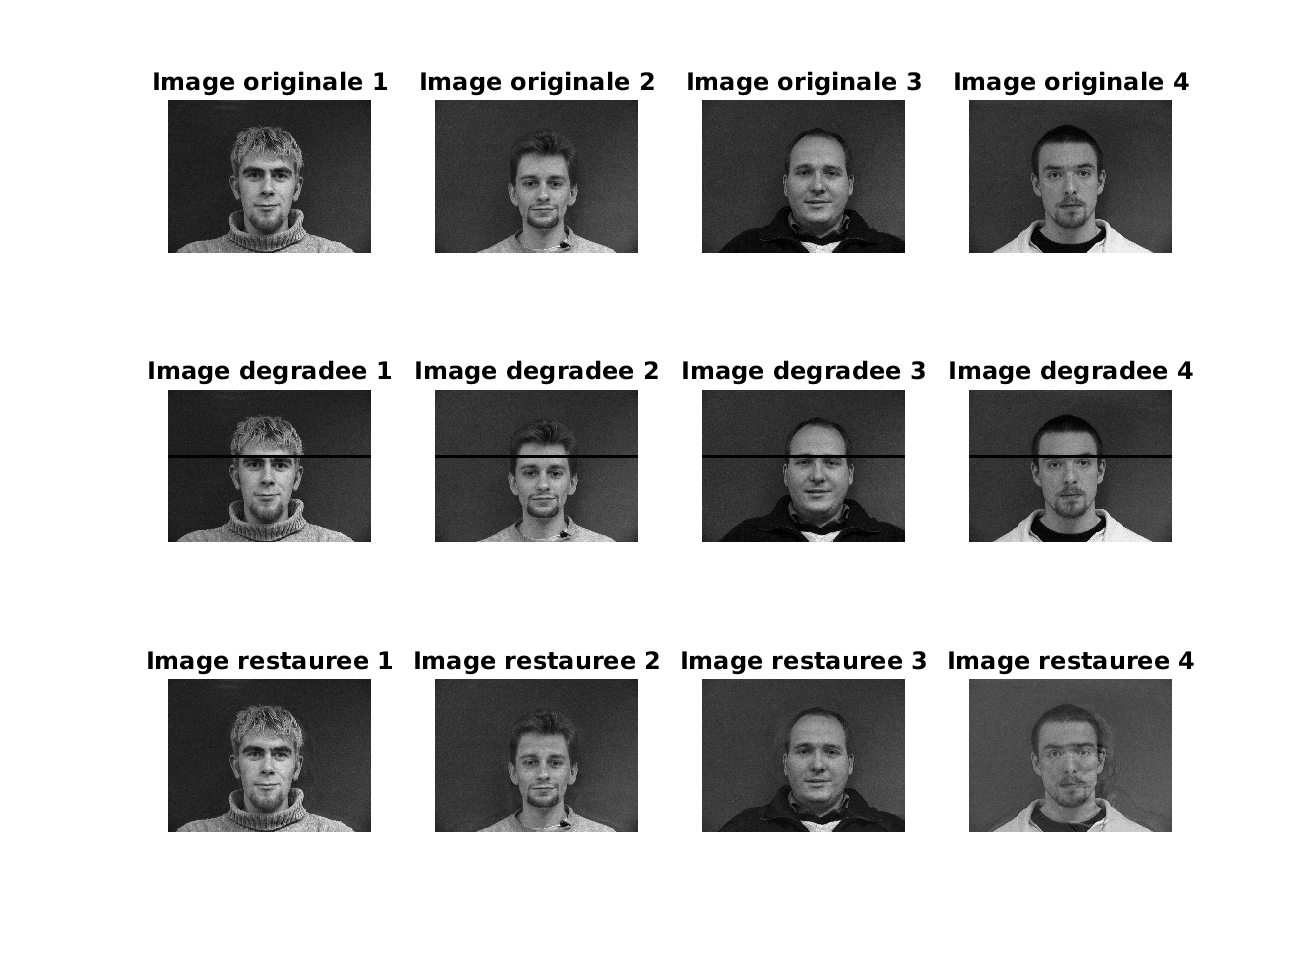
\includegraphics[width=\linewidth]{images/2-bande_5.png}
        \subcaption{Pour une bande noire de 5 pixels d'épaisseur}
    \end{subfigure}
    \begin{subfigure}[c]{0.7\linewidth}
        \centering
        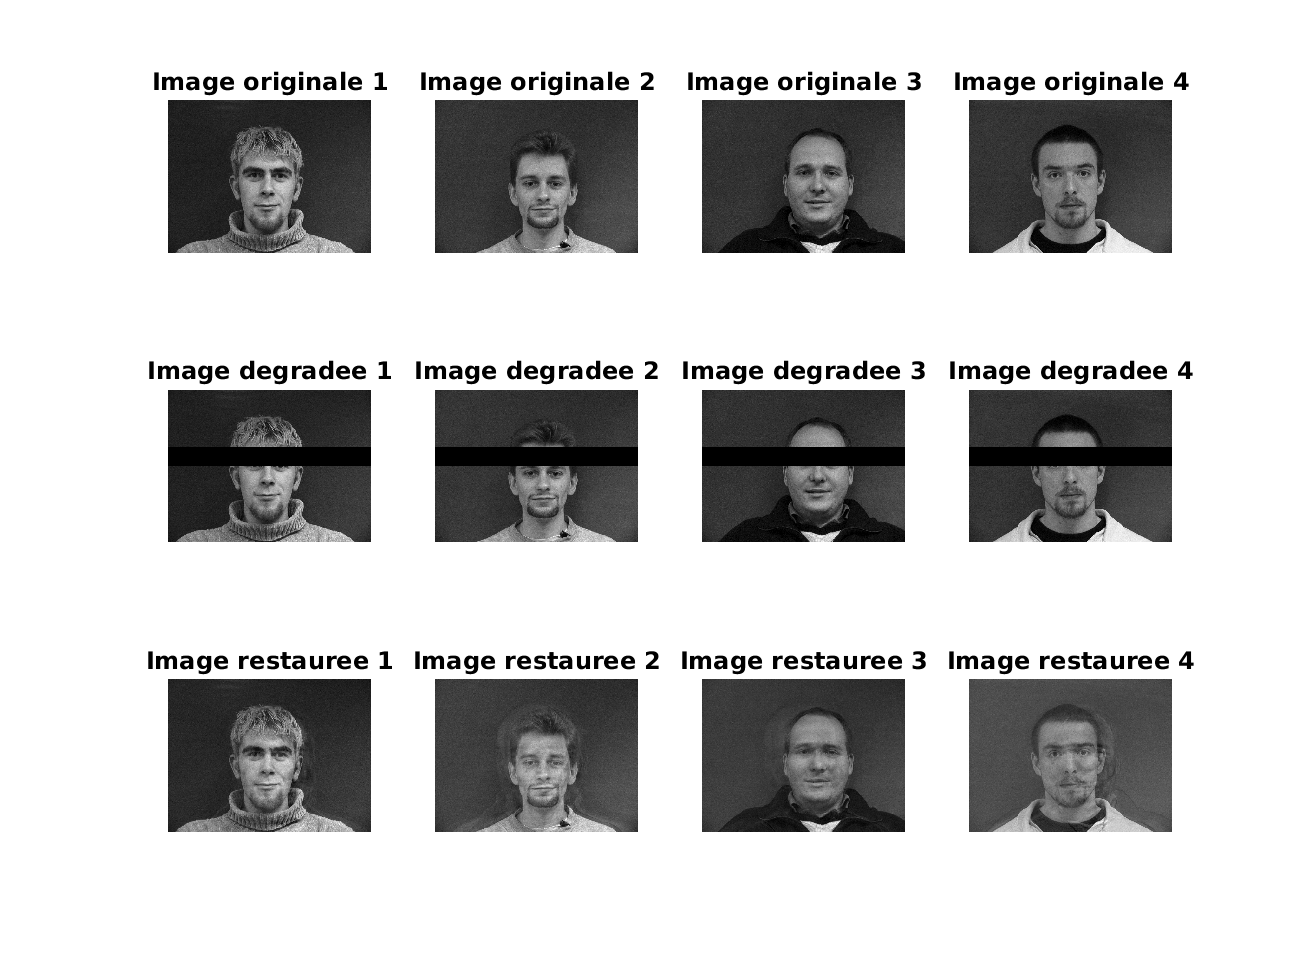
\includegraphics[width=\linewidth]{images/2-bande_30.png}
        \subcaption{Pour une bande noire de 30 pixels d'épaisseur}
    \end{subfigure}
    \caption{Restauration d'images dégradées par des bandes noires}
    \label{reconstitution_bandes_noires}
\end{figure}

\clearpage
\section{TP 3}
\clearpage
\section{TP 4 - Estimation des paramètres d'une ellipse}
Dans ce TP on s'intéresse à l'estimation des paramètres d'une ellipse à partir de l'enregistrement d'une ensemble de ses points. Le but in-fine est par exemple de déterminer l'orientation d'un mur, sur lequel aurait été positionné un cercle, par rapport à l'objectif en estimant les paramètres de l'ellipse alors formée sur l'image.

\subsection{Exercice 1 - Maximum de vraisemblance}
\paragraph{Recherche par tirages aléatoires}
L'idée est donc de trouver une ellipse qui approche au mieux les différents points dont on dispose, ceci en essayant de maximiser la vraisemblance des données observées par rapport à l'ellipse retenue. Pour cela on cherche donc une ellipse qui minimise la distance en norme 2 à l'ensemble des points à notre disposition. Ce premier exercice nous invite à procéder par tirages aléatoires pour trouver une ellipse qui approche les-dits points. On peut voir quelques résultats figure~\ref{3-tirages-aleatoires}.
\begin{figure}[!ht]
    \centering
    \begin{subfigure}[c]{0.49\linewidth}
        \centering
        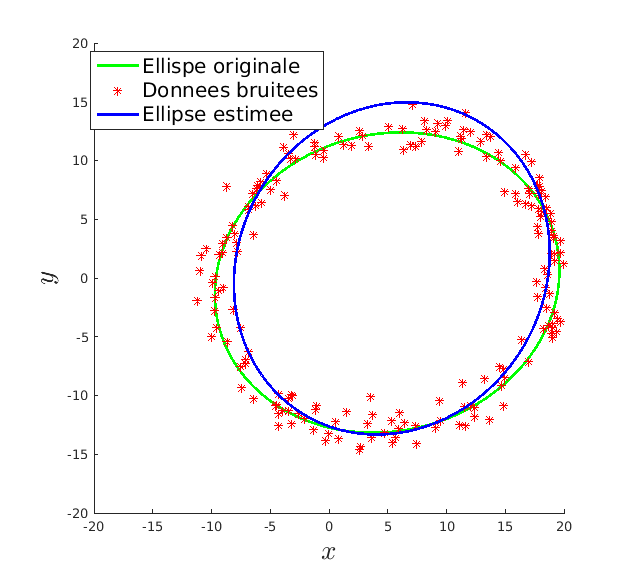
\includegraphics[width=\linewidth]{images/4-hasard_ok.png}
        \subcaption{Erreur de 14.1\%}
    \end{subfigure}
    \begin{subfigure}[c]{0.49\linewidth}
        \centering
        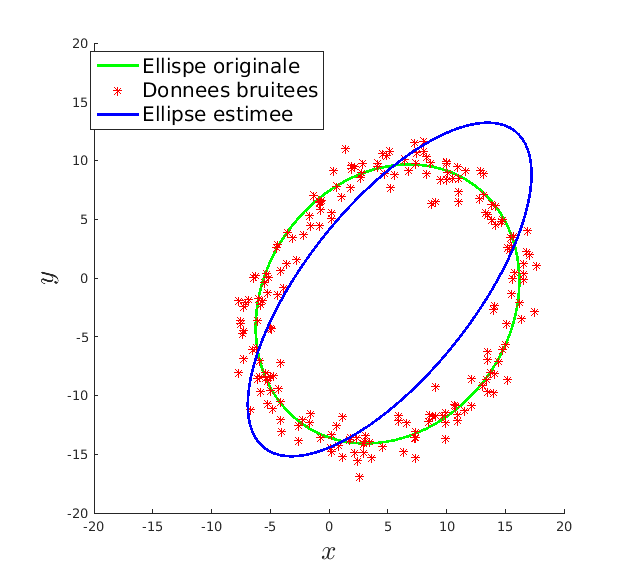
\includegraphics[width=\linewidth]{images/4-hasard_error.png}
        \subcaption{Erreur de 35.1\%}
        \label{3-tirages-aleatoires-erreur}
    \end{subfigure}
    \caption{Estimation d'ellipses par tirages aléatoires}
    \label{3-tirages-aleatoires}
\end{figure}

\paragraph{Résultat très variables}
Cependant on observe aisément que cette méthode n'est pas toujours efficace car elle est sujette au tirage aléatoire auquel nous procédons. Dans la figure~\ref{3-tirages-aleatoires-erreur} on voit par exemple que l'ellipse estimée est très loin de celle originale. L'erreur faite peut alors très fortement varier et se situe en moyenne pour 500 tirages aux alentours de 0.2.

\subsection{Exercice 2 - Moindres carrés ordinaires}
\paragraph{Système linéaire issu de l'équation d'une conique et d'une contrainte linéaire}
Dans un deuxième temps on s'intéresse à l'équation cartésienne de l'ellipse, celle qui est commune avec les autres coniques. Si celle-ci fait jouer 6 paramètres, deux sont pourtant liés dans le cas de l'ellipse car celle-ci ne demande que 5 paramètres pour être définie. Ainsi on propose de rajouter une contraintes (soit $\alpha + \gamma = 1$ soit $\Phi = 1$) puis de résoudre approximativement le système linéaire sur-contraint au sens des moindres carrés ordinaires. On obtient alors les résultats de la figure~\ref{3-moindres-carres-ordinaires} pour les deux contraintes envisagées.
\begin{figure}[!ht]
    \centering
    \begin{subfigure}[c]{0.49\linewidth}
        \centering
        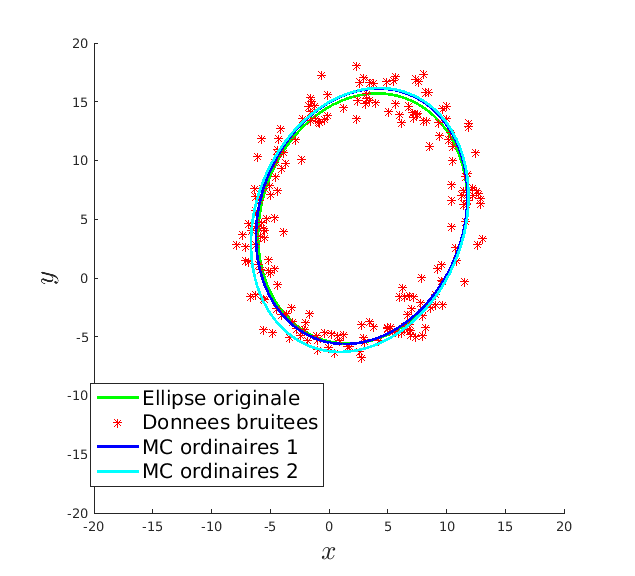
\includegraphics[width=\linewidth]{images/4-mco_1.png}
        \subcaption{Erreurs de 3.7\% et 8.3\%}
    \end{subfigure}
    \begin{subfigure}[c]{0.49\linewidth}
        \centering
        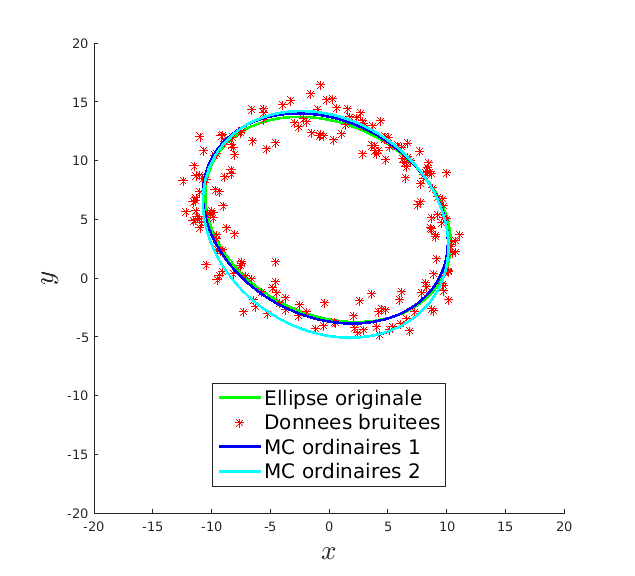
\includegraphics[width=\linewidth]{images/4-mco_2.png}
        \subcaption{Erreurs de 4\% et 10.5\%}
    \end{subfigure}
    \caption{Estimation d'ellipses par tirages aléatoires}
    \label{3-moindres-carres-ordinaires}
\end{figure}

\paragraph{Erreur}
Ici l'erreur faite par rapport à l'ellipse originale varie quelque peu mais se trouve généralement aux alentours de 3\% pour la première contrainte et de 9\% pour la deuxième contrainte.

\subsection{Exercice 3 - Moindres carrés totaux}
\paragraph{Contrainte non linéaire et problème de minimisation induit}
Dans le but d'éviter les problèmes de non résolvabilité induits par les contraintes linéaires proposées dans l'exercice précédent, on s'intéresse ici à la même équation de conique à laquelle on rajoute la contrainte $||X|| = 1$ qui n'est cette fois ci pas linéaire. Le problème de minimisation admet alors toujours une solution et c'est la théorie Lagrangienne qui nous permet de la trouver. Après implémentation de l'algorithme, on obtient les résultats de la figure~\ref{3-moindres-carres-totaux}.
\begin{figure}[!ht]
    \centering
    \begin{subfigure}[c]{0.49\linewidth}
        \centering
        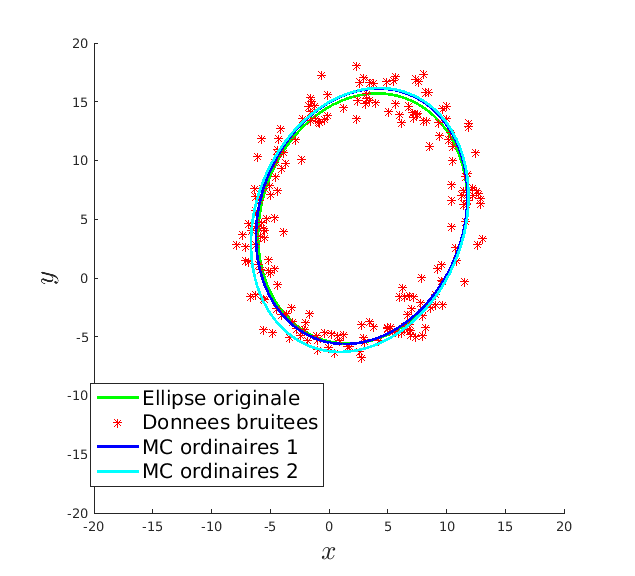
\includegraphics[width=\linewidth]{images/4-mco_1.png}
        \subcaption{Erreurs de 2.2\%, 2.5\%, et 2.5\%}
    \end{subfigure}
    \begin{subfigure}[c]{0.49\linewidth}
        \centering
        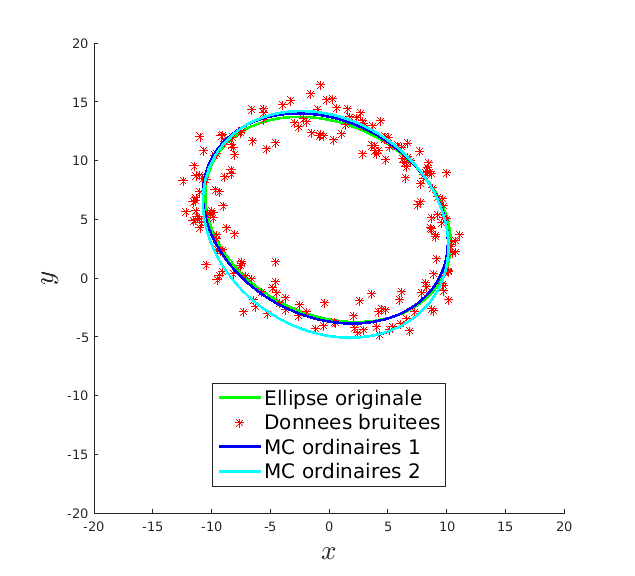
\includegraphics[width=\linewidth]{images/4-mco_2.png}
        \subcaption{Erreurs de 5.3\%, 15.6\%, et 14.9\%}
    \end{subfigure}
    \caption{Estimation d'ellipses par tirages aléatoires}
    \label{3-moindres-carres-ordinaires}
\end{figure}

\paragraph{Erreur}
Assez surpris j'observe que dans ce cas l'erreur est souvent supérieure à celle obtenue pour le cas des moindres carrés ordinaires dans le cas de la contrainte $\alpha + \gamma = 1$. En effet je m'attendais à trouver une erreur meilleur puisque la contrainte semble moins contraignante, mais ça n'est pas le cas. Elle se situe aux alentours de 7\%. Finalement les erreurs moyennes pour les différentes méthodes par moindres carrés sont :
\begin{itemize}
    \item $\alpha + \gamma = 1$ : 4\%
    \item $\Phi = 1$ : 9\%
    \item $||X|| = 1$ : 7\%
\end{itemize}
On observe aussi que l'erreur faite par l'algorithme des moindres carrés ordinaires sous la première contrainte est bien plus constantes que pour les autres algorithmes.

\paragraph{Application à la réalité augmentée}
Pour l'application à la réalité augmenté j'ai choisi de prendre le risque de rendre le système sans solution en utilisant la méthode des moindres carrés ordinaires sous la contrainte $\alpha + \gamma = 1$ puisque c'est celle qui m'a donné les résultats les plus précis et les plus constants. J'ai misé en outre sur le fait qu'il n'est finalement pas si probable de tomber dans un cas où le problème n'admet pas de solution. J'ai alors obtenu des résultats très concluants.

\section{TP 5 - Détection de la ligne d'horizon dans une image}
Ce TP traite de la détection de lignes dans une image et de comment cela peut être utilisé pour obtenir ses points de fuites et ainsi retrouver sa ligne d'horizon.

\subsection{Exercice 1 - Transformation de Hough}
\paragraph{Détection des lignes d'une image}
Dans un premier temps on s'intéresse à la détection des lignes d'une image. Pour ce faire on commence par trouver les contours dans l'image (algorithmes vus en traitement d'image, résultat figure~\ref{5-contours}) puis on tente, par transformation de Hough, de placer des droites dans l'image qui passent par le plus de points de contours possible. L'idée est assez simple et consiste à paramétriser des droites par leur angle avec l'axe des abcisse et leur distance à une origine quelconque.
\begin{figure}[!ht]
    \centering
    \begin{subfigure}[c]{0.49\linewidth}
        \centering
        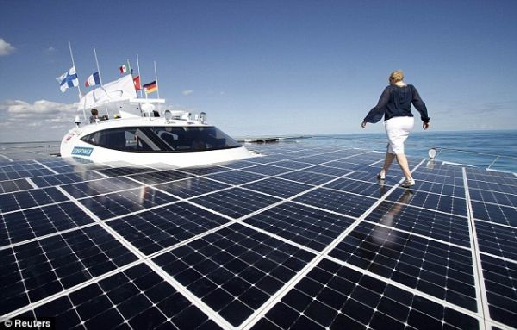
\includegraphics[width=\linewidth]{images/5-original.png}
    \end{subfigure}
    \hfill
    \begin{subfigure}[c]{0.49\linewidth}
        \centering
        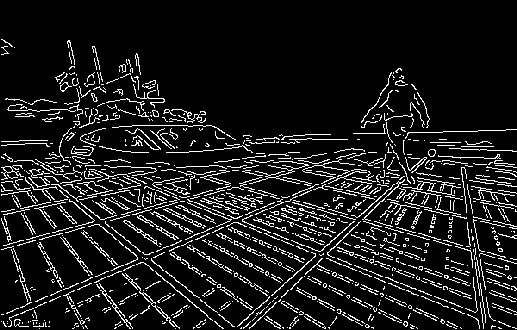
\includegraphics[width=\linewidth]{images/5-contours.png}
    \end{subfigure}
    \caption{Image originale et ses contours par transformation de Hough}
    \label{5-contours}
\end{figure}

\paragraph{La matrice C}
Durant cet exercice on introduit la matrice C. Celle-ci contient le nombre de points de contours par lesquels passent les droites paramètrées par les différentes valeurs de $\theta$ et $\rho$ respectivement en abcisse et en ordonnée. On peut voir une représentation de cette matrice figure~\ref{5-C}.
\begin{figure}
	\centering
	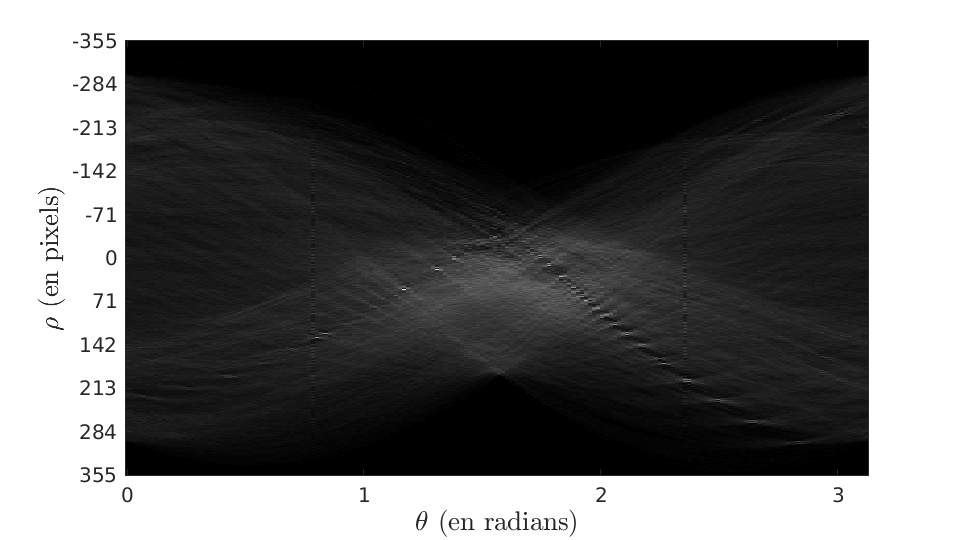
\includegraphics[width=0.7\linewidth]{images/5-C.png}
	\label{5-C}
	\caption{Matrice présences des droites dans l'image}
\end{figure}

\subsection{Exercice 2 - Maxima locaux de la matrice C}
\paragraph{Choix des lignes}
Pour choisir les lignes à conserver, c'est à dire celles qui suivent réellement des contours de l'image, il faut procéder avec précaution car on pourraît être amené à choisir deux lignes très proches (donc n'apportant que peu de détail nouveau) si on sélectionne uniquement celles ayant obtenu le meilleur score. L'idée est donc de sélectionner une à une les lignes de plus grand score tout en prenant soin d'annuler le score de ces lignes et de celles qui leur sont trop proches à mesure qu'on les sélectionne. Pour cela on choisi un maximum de C, on annule une petite zone autour de ce maximum, et on recommence. On conserve alors un nombre arbitraire n de lignes comme on peut le voir figure~\ref{5-lignes}.
\begin{figure}[!ht]
    \centering
    \begin{subfigure}[c]{0.49\linewidth}
        \centering
        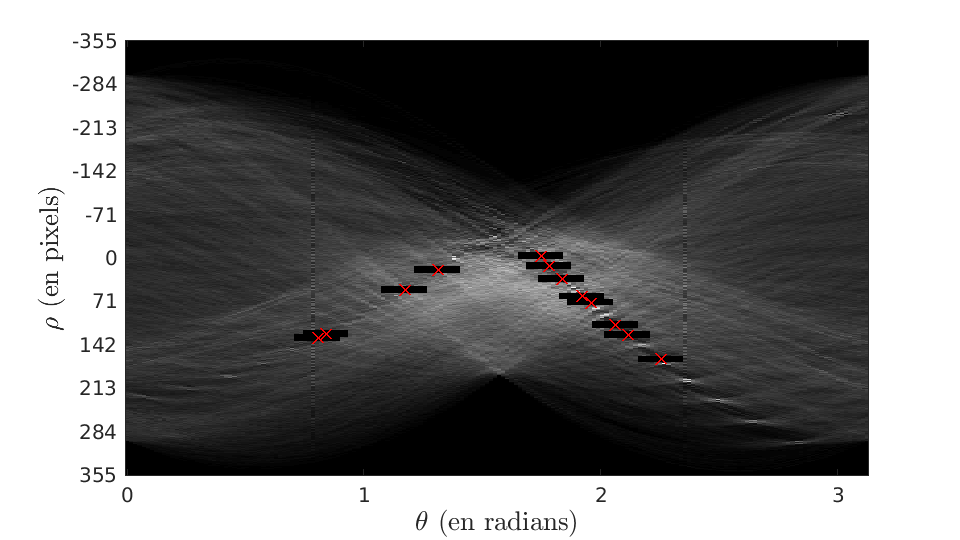
\includegraphics[width=\linewidth]{images/5-C_lines.png}
    \end{subfigure}
    \hfill
    \begin{subfigure}[c]{0.49\linewidth}
        \centering
        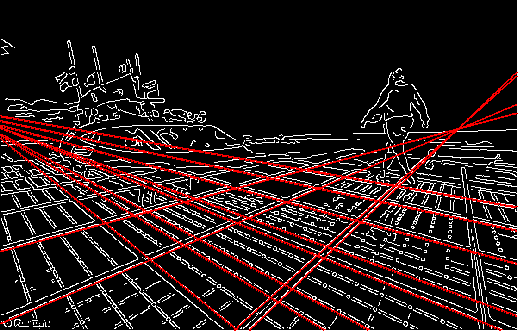
\includegraphics[width=\linewidth]{images/5-lines.png}
    \end{subfigure}
    \caption{Détections des lignes dans l'image par maxima locaux de C}
    \label{5-contours}
\end{figure}

\paragraph{Zone de C à annuler}
Lorsque l'on choisi une ligne, on s'empèche de prendre celles voisines. Il faut faire attention à annuler une zone suffisament grande pour ne pas faire un calcul des points de fuite erroné plus tard, mais pas trop sinon on risque de perdre de l'information. On peut par exemple voir ce qui arrive avec une fenêtre trop petite figure~\ref{5-T-petit} et avec une fenêtre trop grande figure~\ref{5-T-grand}. Dans le premier cas les lignes trouvées se chevauchent car pour une même ligne réelle correspondent plusieurs couple $(\rho, \theta)$ (car l'image est constituée de pixels donc c'est approximatif); dans le deuxième cas des lignes peu intéressante sont découverte car la fenêtre en masque trop.
\begin{figure}[!ht]
    \centering
    \begin{subfigure}[c]{0.49\linewidth}
        \centering
        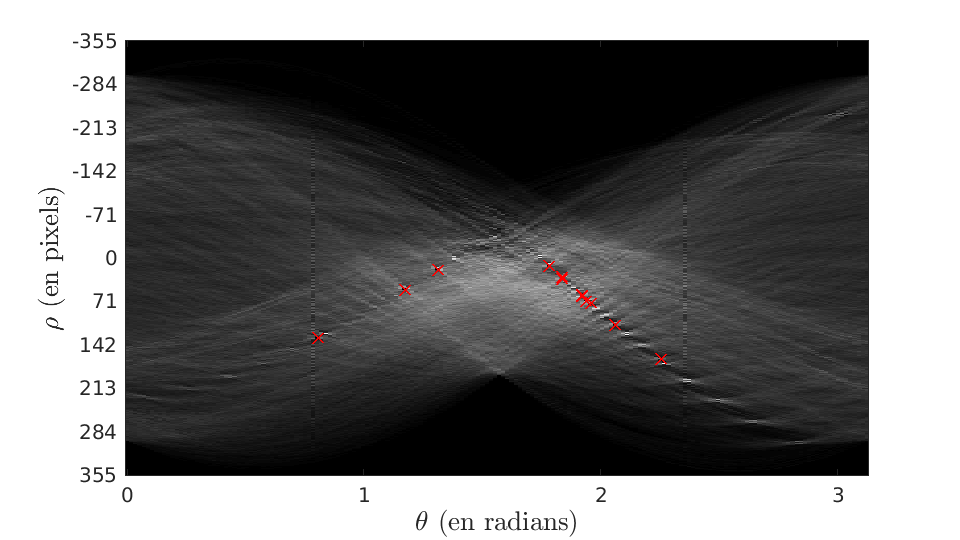
\includegraphics[width=\linewidth]{images/5-C_Tpetit.png}
    \end{subfigure}
    \hfill
    \begin{subfigure}[c]{0.49\linewidth}
        \centering
        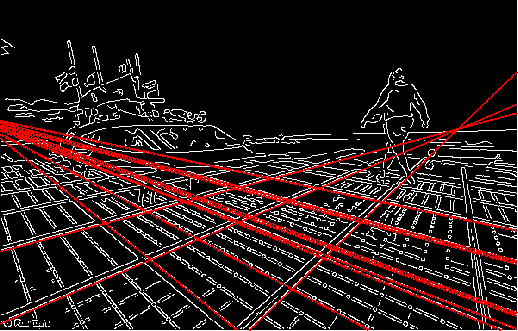
\includegraphics[width=\linewidth]{images/5-lines_Tpetit.png}
    \end{subfigure}
    \caption{Détections des lignes avec une petite fenêtre T (1)}
    \label{5-T-petit}
\end{figure}
\begin{figure}[!ht]
    \centering
    \begin{subfigure}[c]{0.49\linewidth}
        \centering
        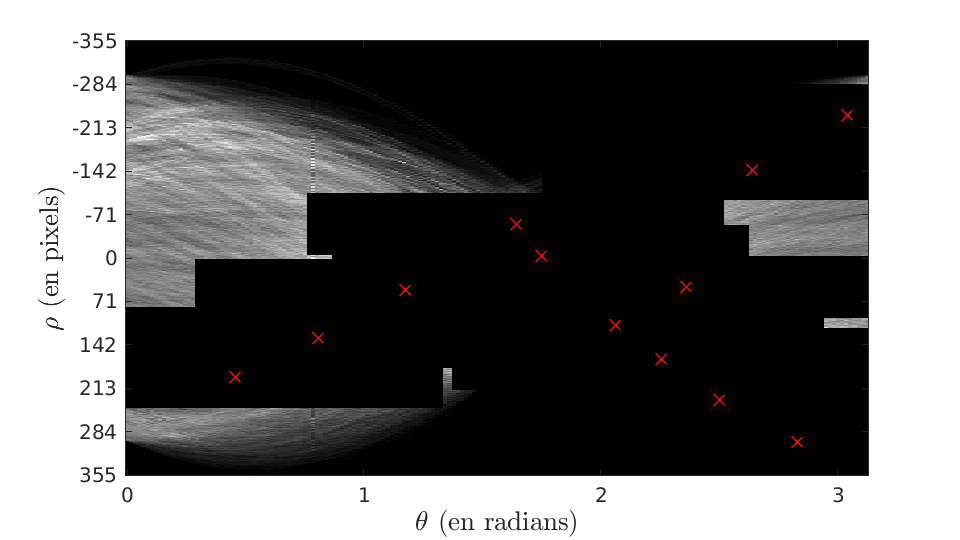
\includegraphics[width=\linewidth]{images/5-C_Tgrand.png}
    \end{subfigure}
    \hfill
    \begin{subfigure}[c]{0.49\linewidth}
        \centering
        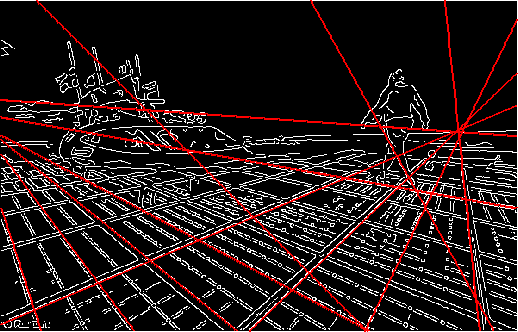
\includegraphics[width=\linewidth]{images/5-lines_Tgrand.png}
    \end{subfigure}
    \caption{Détections des lignes avec une grande fenêtre T (50)}
    \label{5-T-grand}
\end{figure}
Dans tous les cas si on ne récolte pas les bonnes lignes on aura des points de fuites mal positionnés et cela faussera le résultat. On choisit donc $T=5$ bien qu'on aurait pu faire le choix de T de manière plus fine en tenant compte de la différence d'homogénéité entre les deux paramètres.


\subsection{Exercice 5 - Localisation des points de fuite}
\paragraph{Les points de fuite}
Dans une image, les droites parallèles et orthogonales d'un plan devraient se croiser en deux points de fuite. Un tel point de fuite se trouvant alors sur plusieurs droites, il vérifie pour celles-ci :
\[\rho = \rho_Fcos(\theta - \theta_F)\]
où $\rho_F$ et $\theta_F$ sont les coordonnées polaires du point de fuite et $\rho$ et $\theta$ les coordonnées de la droite considérée. De cette façon l'ensemble des droites passant par ces points de fuitent devraient se répartir sur la matrice C selon une courbe sinusoïdale (deux en fait, une pour chaque point de fuite) et c'est bien le cas.

\paragraph{Scinder les droites en deux classes}
Il se trouve que, par hasard, les droites dans l'image sont principalement orientées selon des angles d'environ 45 degré. De cette façon, et dans ce cas uniquement, les points dans C de ces droites sont principalement positionnés sur des parties "droites" des courbes sinusoïdales. Ainsi on peut trouver deux droites dans la matrice C de façon à ce que chaque point retenu passe par l'une ou l'autre de ces deux droites, ou encore plus simplement - puisque de toute façon on fait déjà une hypothèse forte - remarquer que les droites sont séparable selon le signe de l'angle $\theta - \pi/2$ qui les paramètre puisque l'origine du repère a été choisie entre les deux points de fuite de l'image. On obtient alors la répartition figure~\ref{5-repartition}.
\begin{figure}[!ht]
    \centering
    \begin{subfigure}[c]{0.49\linewidth}
        \centering
        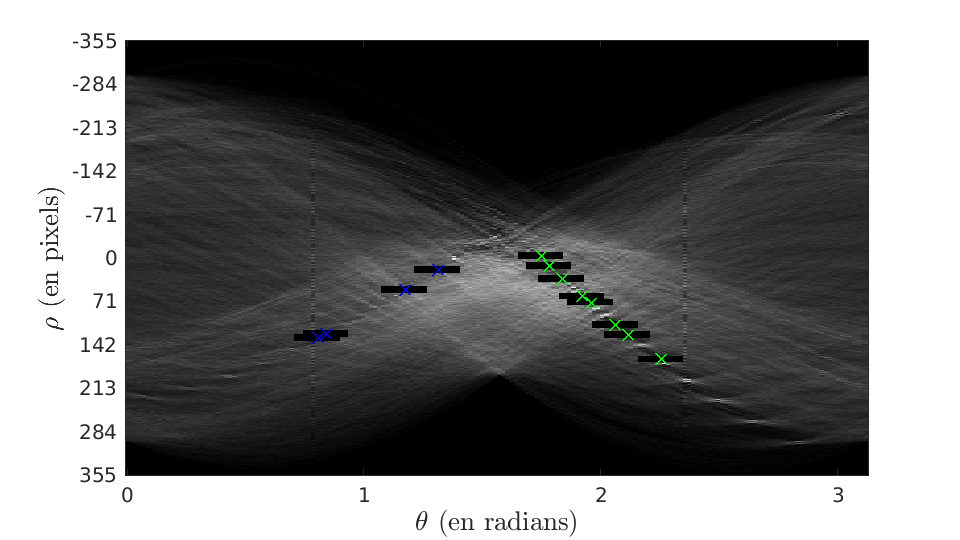
\includegraphics[width=\linewidth]{images/5-C_repartition.png}
    \end{subfigure}
    \hfill
    \begin{subfigure}[c]{0.49\linewidth}
        \centering
        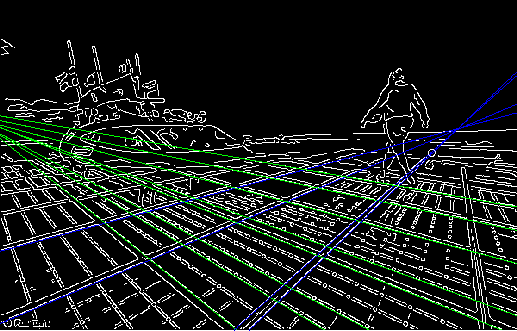
\includegraphics[width=\linewidth]{images/5-lines_repartition.png}
    \end{subfigure}
    \caption{Répartition des droites selon les deux points de fuite}
    \label{5-T-grand}
\end{figure}

\paragraph{Ligne d'horizon}
Pour conclure on relie les deux points de fuite et on s'apperçoit que, malgré le calme apparent de la mer, le bateau n'était pas vraiment à l'horizontal lors de la prise de vue, l'horizon "visuel" ne correspondant pas avec celui calculé (figure~\ref{5-horizon}).
\begin{figure}[!ht]
    \centering
    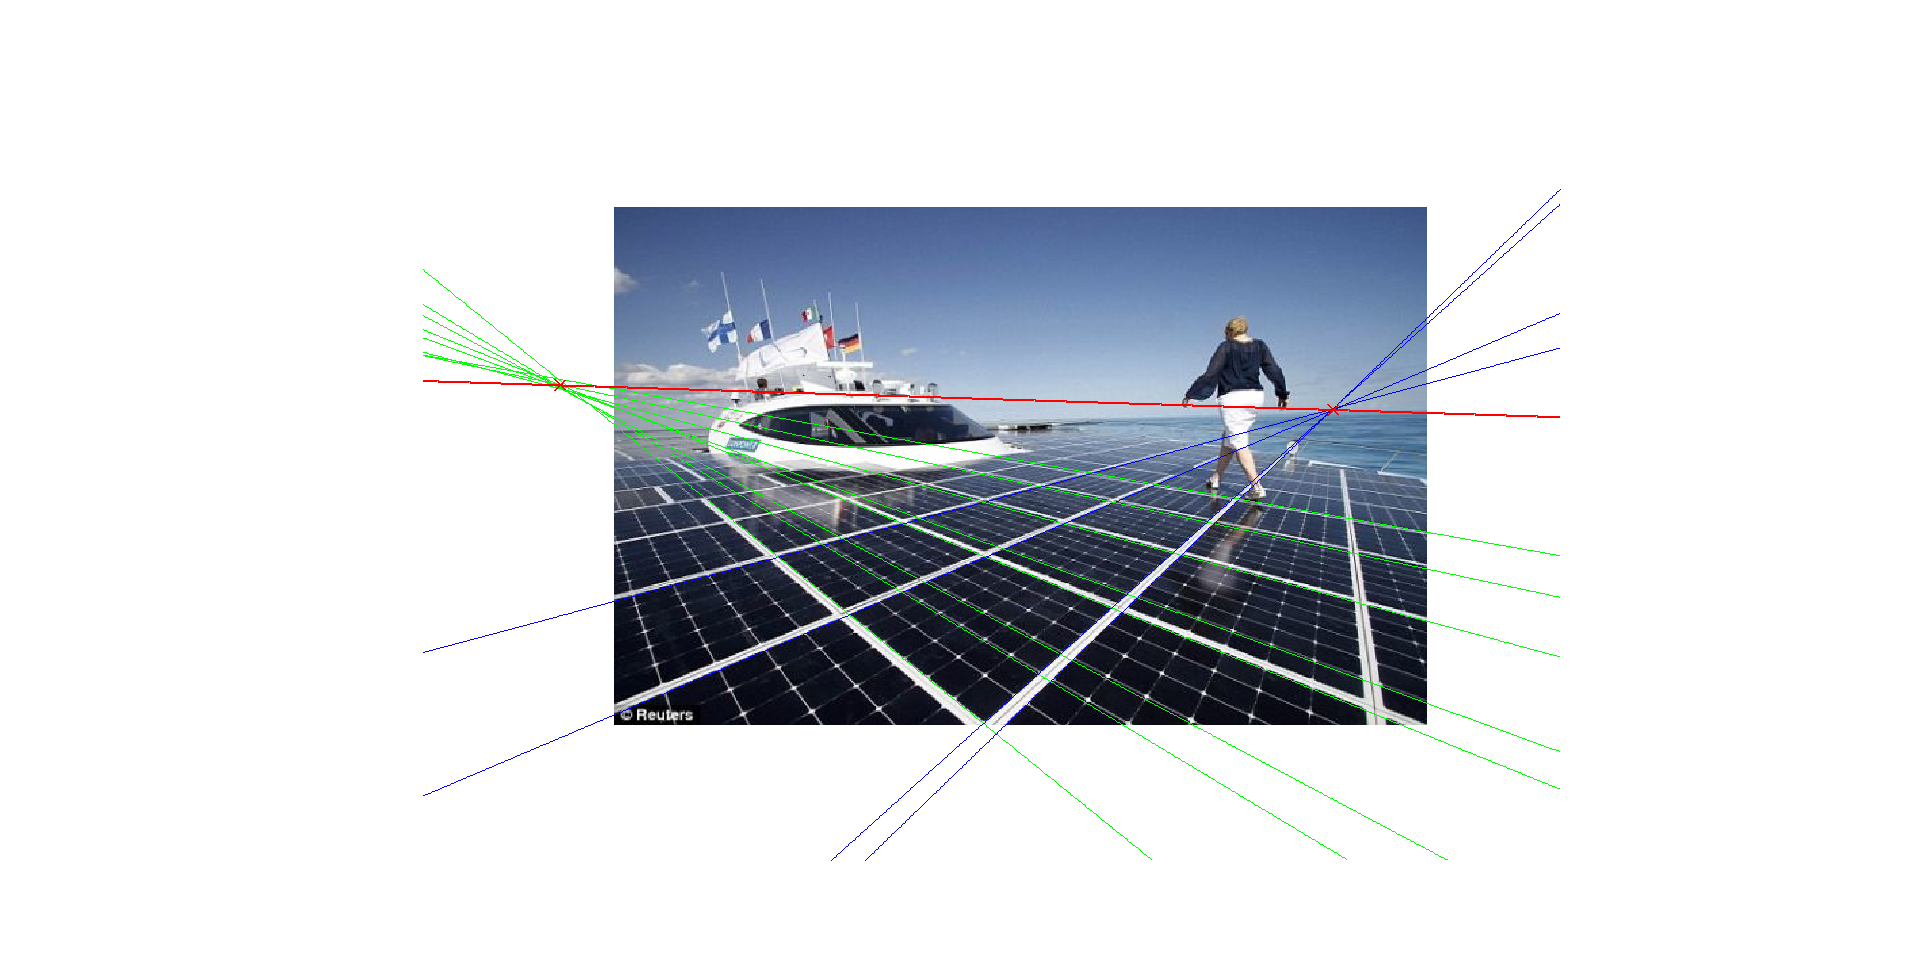
\includegraphics[width=\linewidth]{images/5-houle.png}
    \caption{Visualisation de la ligne d'horizon}
    \label{5-horizon}
\end{figure}

\clearpage
\section{TP 6 - Détection et comptage d'objets}
Comme son titre l'indique, ce TP nous intéresse à la détection et au comptage d'objets dans une image. En particulier on essaye de compter des flamants rose sur une image noir et blanc.

\subsection{Exercice 0 - Algorithme naïf}
\paragraph{Remarque}
Les premiers algorithmes consistent à positionner correctement au mieux un nombre N donné de disques à l'endroit où l'on suspecte la position d'un flamant rose. On s'intéressera qu'à la fin du TP à l'augmentation et à la diminution de ce chiffre N de manière dynamique.

\paragraph{Algorithme naïf}
Cet exercice préliminaire qu'il nous est juste demandé d'exécuter est là pour nous faire remarquer les défauts de la recherche naïve qui consiste à placer des disques là où on pense trouver un flamant rose, mais ce de manière indépendante d'un disque à l'autre. On obtient alors le résultat figure~\ref{6-naif} qui donne un niveau de gris moyen de 220 environ.
\begin{figure}[!ht]
    \centering
    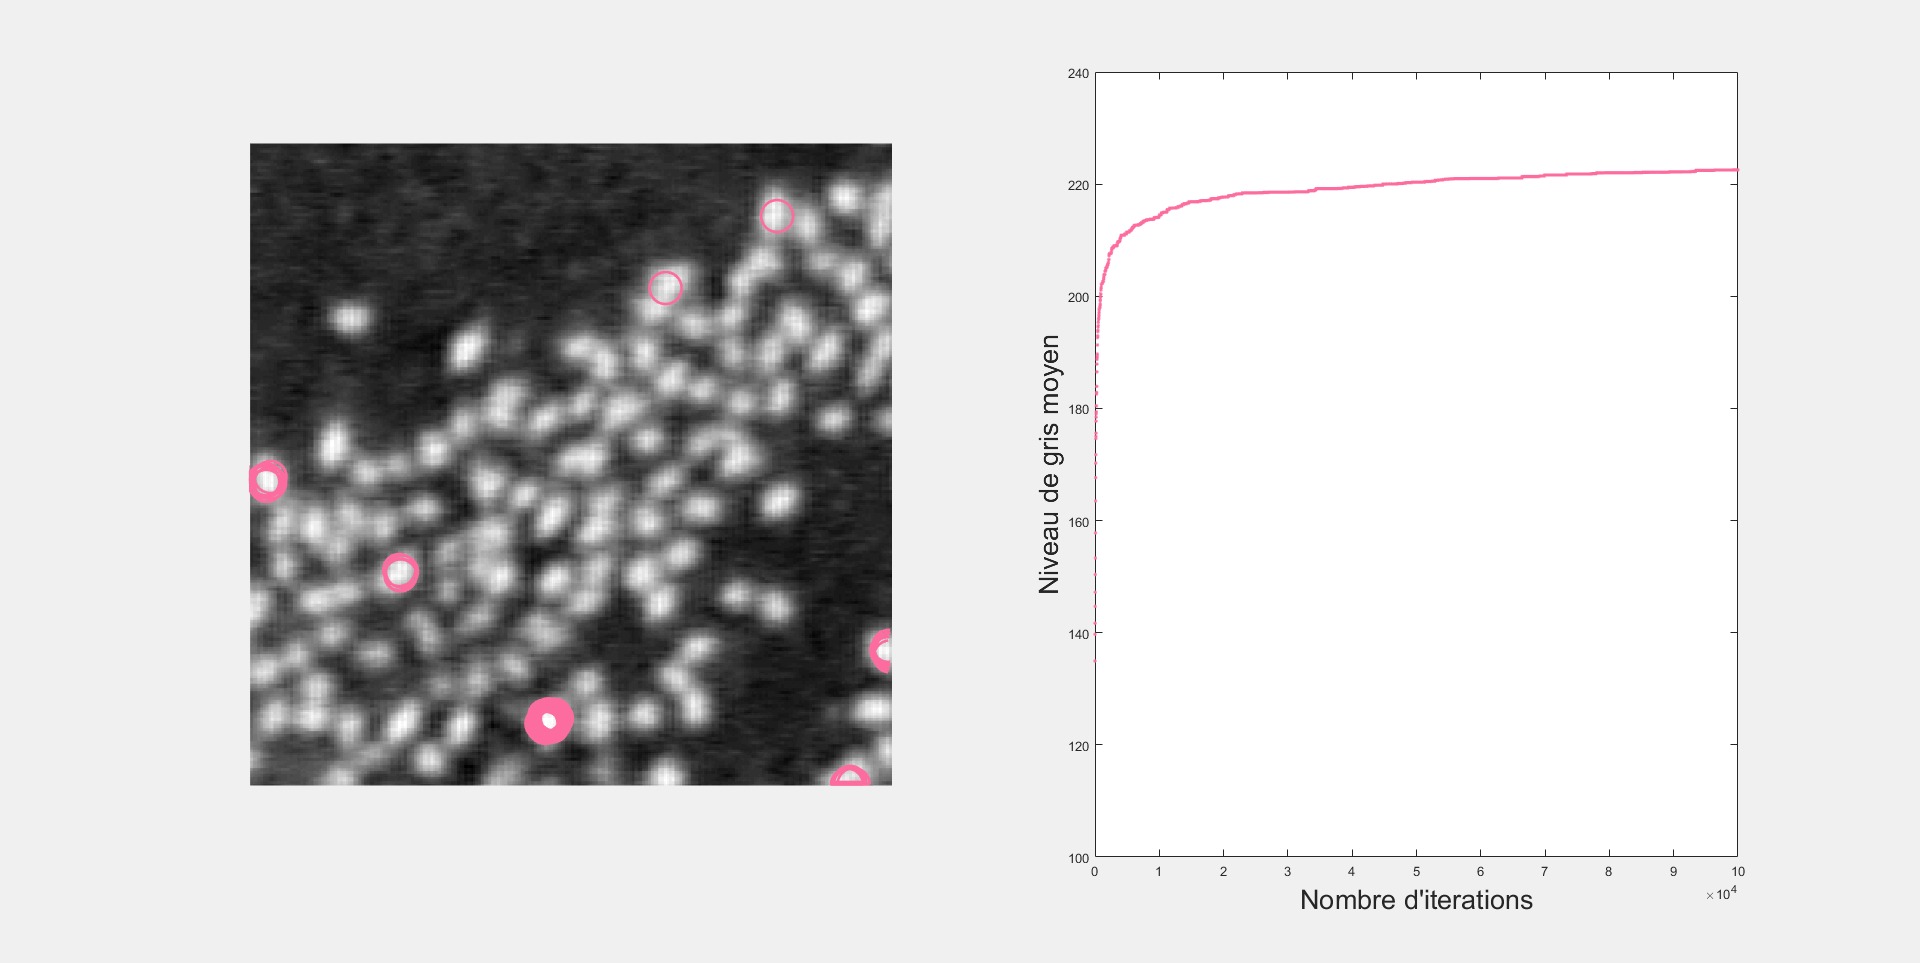
\includegraphics[width=\linewidth]{images/6-naif.png}
    \caption{Algorithme aléatoire naïf}
    \label{6-naif}
\end{figure}

Le soucis relevé par cette méthode est que chaque disque va essayer, indépendament de la position des autres, de se positionner là où le niveau de gris de l'image est le plus élevé. Cette non dépendance entre les disques entraine que in-fine tous les disques devraient se retrouver exactement au même endroit. Il apparaît donc comme nécessaire d'empêcher les disques de se chevaucher, c'est ce qu'on fera par la suite.

\subsection{Exercice 1 - Champ de Markov}
\paragraph{Prévenir le recouvrement des disques}
Dans un deuxième temps on cherche donc à maîtriser la distance entre deux disques pour éviter qu'ils se chevauchent et se retrouvent donc au même endroit. En imposant une distance minimale entre les disques, qui leur permet néanmoins de se chevaucher partiellement, on obtient des résultats bien plus intéressants que l'on peut observer figure~\ref{6-markov}. Cette fois ci le niveau de gris moyen est d'environ 180 (la baisse par rapport à l'algorithme naïf est parfaitement cohérente).
\begin{figure}[!ht]
    \centering
    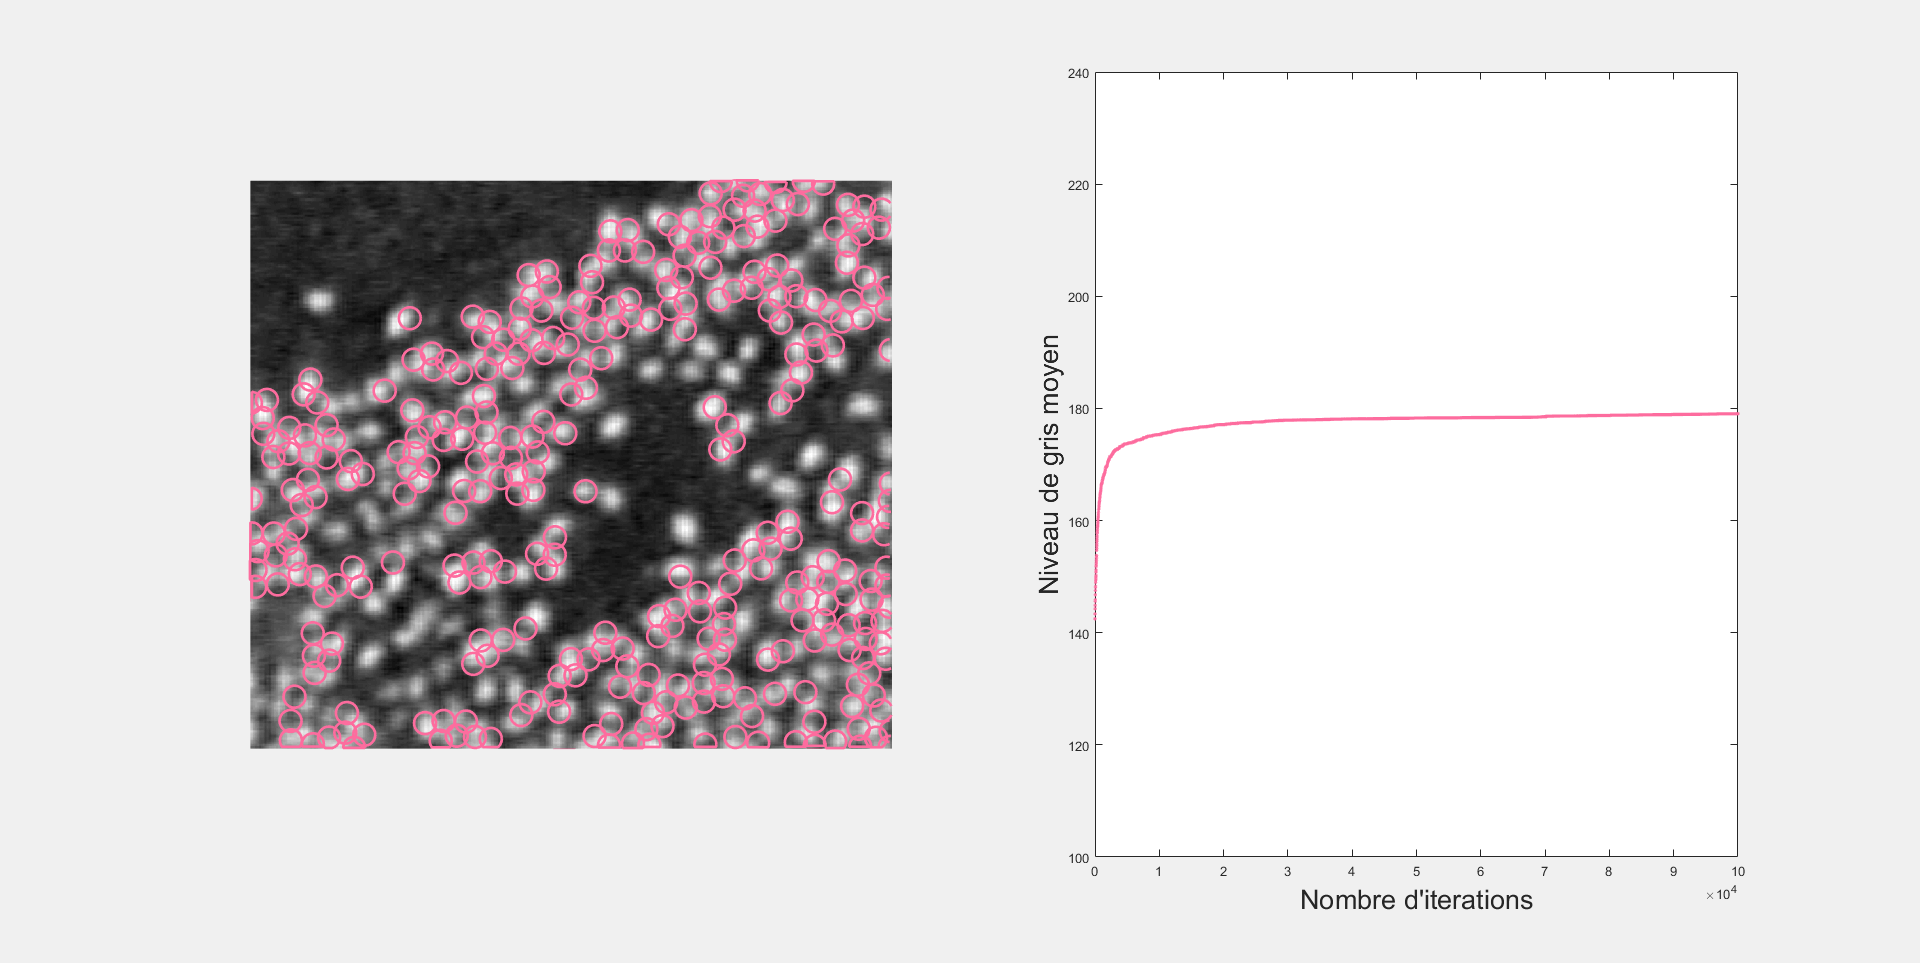
\includegraphics[width=\linewidth]{images/6-markov.png}
    \caption{Algorithme par champs de Markov}
    \label{6-markov}
\end{figure}

\paragraph{Le nombre de flamants rose}
Le principal problème de cette méthode est qu'elle impose de donner à priori le nombre de flamants roses dans l'image, l'algorithme se contentant simplement de les placer correctement. Il faut donc le relancer plusieurs fois avec des paramètres différents pour obtenir un résultat concluant.

\subsection{Exercice 2 - Processus ponctuel marqué}
\paragraph{Principe}
Le principe du décompte de flamants roses par processus ponctuel marqué est de calculer l'énergie d'une configuration et de chercher à la minimiser, cette énergie étant la somme d'un terme d'attache aux données (est-ce que le disque est placé sur un flamant rose ?) et d'un terme d'a priori (est-ce qu'un disque identifie déjà ce flamant rose ?). En jouant sur les paramètres et sur le rapport de ces deux termes, on espère parvenir à compter le nombre de flamants roses.

\paragraph{Naissances et morts multiples}
Si l'on s'en tient au processus ponctuel marqué, on ne corrige pas le problème du nombre de flamants roses à trouver. L'initiative retenue est donc de rajouter à chaque itération un certain nombre de disques puis de retirer ceux les moins bien placés.

\paragraph{Résultat}
Après implémentation de l'algorithme complet, on obtient le résultat figure~\ref{6-marque}, qui compte 356 flamants roses. Cependant il faut au préalable jouer sur les différents paramètres ($\beta$ pour donner plus ou moins d'importance au recouvrement des disques, $S$ pour déterminer la taille a priori d'un flamant rose, $\gamma$ pour jouer sur l'intérêt porté à la couleur des flamants (plus $\gamma$ est élevé, moins l'image nécessite d'être contrastée pour détecter correctement les flamants roses), $T_0$ pour jouer sur le nombre de naissances initial, $\lambda_0$ pour jouer sur la vitesse initiale de variation du nombre de naissances et de morts, et $\alpha$ pour jouer sur la variation au cours du temps de la vitesse de changement du nombre de naissances et de morts).
\begin{figure}[!ht]
    \centering
    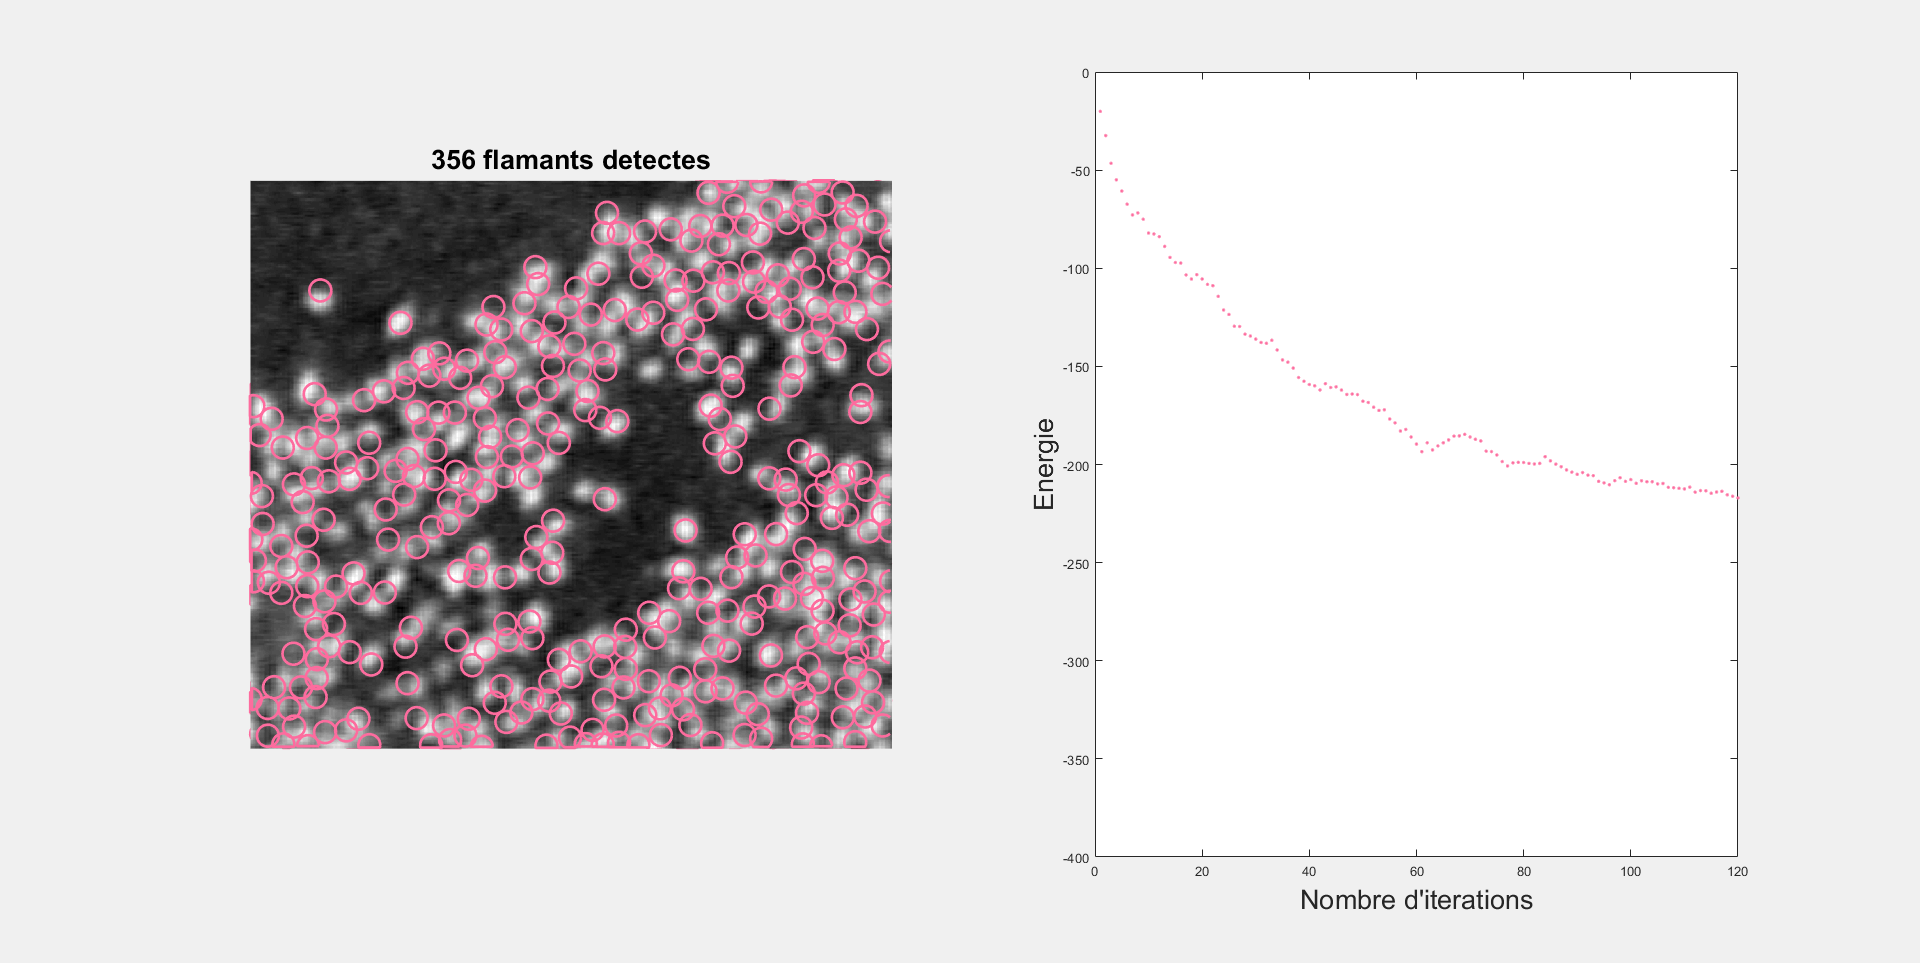
\includegraphics[width=\linewidth]{images/6-best.png}
    \caption{Comptage par naissances et morts multiples}
    \label{6-naif}
\end{figure}

\paragraph{Remarques}
L'algorithme est très lent à converger puisqu'il effectue 120 itérations de naissances et morts. L'énergie finale est alors d'environ -215.


\section{TP 7 - Contours actifs}
Le but de ce TP est d'étudier l'algorithme du contour actif qui permet d'isoler le contour d'une forme dans une image.

\subsection{Introduction}
Il s'agit d'un problème qui peut se mettre sous une forme variationnelle pour laquelle on connaît un moyen de résolution. Il faut donc commencer par modéliser le problème puis entamer la résolution, comme le propose le sujet dans une étude préliminaire.

\subsection{Exercice 1 - Énergie externe}
\paragraph{Énergie externe}
L'équation $E_{ext}(P(s)) = - ||\nabla I(P(s))||^2$ défini l'énergie $E_{ext}$ qu'il nous faut minimiser pour résoudre le problème variationnel associé à la détection de contours. On commence donc par afficher, pour une image donnée, la valeur de cette énergie en tous points (figure~\ref{7-energie}). On remarque ici que loin des contours réels dans l'image cette énergie est très faible (puisqu'elle dépend du gradient qui y est nul) ce qui fait qu'un snake mal initialisé pourraît ne pas bouger (ne sachant pas dans quelle direction se déplacer).
\begin{figure}[!ht]
    \centering
    \begin{subfigure}[c]{0.32\linewidth}
        \centering
        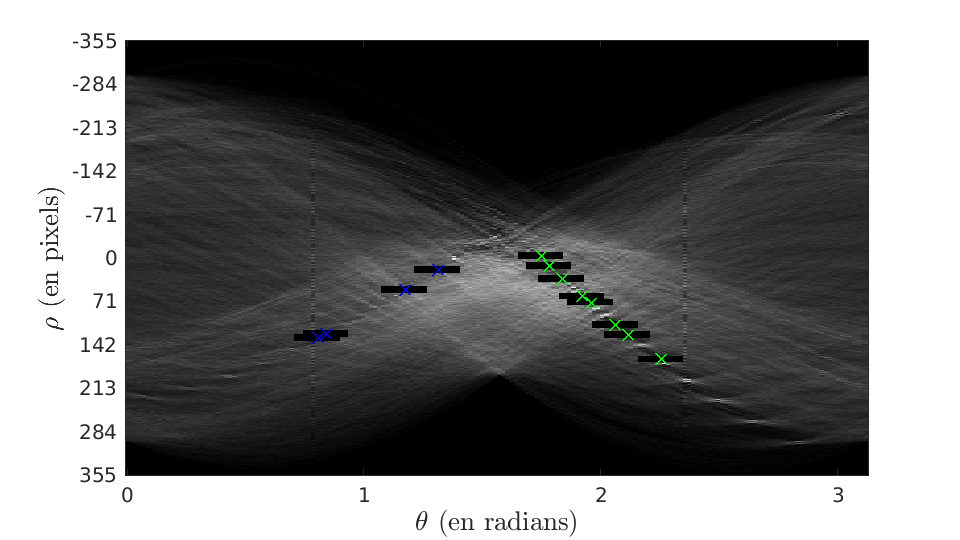
\includegraphics[width=\linewidth]{images/5-C_repartition.png}
    \end{subfigure}
    \hfill
    \begin{subfigure}[c]{0.32\linewidth}
        \centering
        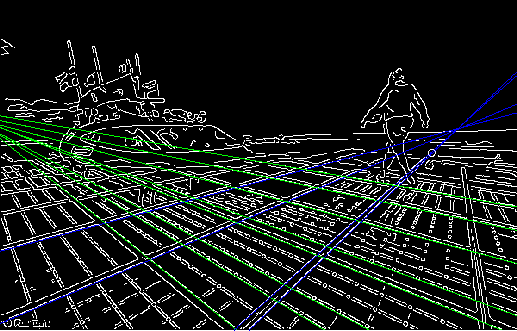
\includegraphics[width=\linewidth]{images/5-lines_repartition.png}
    \end{subfigure}
    \caption{Répartition des droites selon les deux points de fuite}
    \label{5-T-grand}
\end{figure}

\paragraph{Solution}
La solution proposée par le sujet consiste donc à appliquer un flou gaussien à l'image pour étaler les zones de contours de façon à étaler les zones de variation de l'énergie externe. On obtient alors le résultat présenté figure~\ref{7-gaussien}. De cette façon si le flou gaussien est peu étalé (T trop petit) alors on aura le même problèème que précédemment et inversement si il est trop étalé ou trop prononcé (T grand ou $\sigma$ grand) alors les zones d'énergie élevée seront trop étalées ce qui rendra le mouvement du contour pas assez important.

\begin{figure}[!ht]
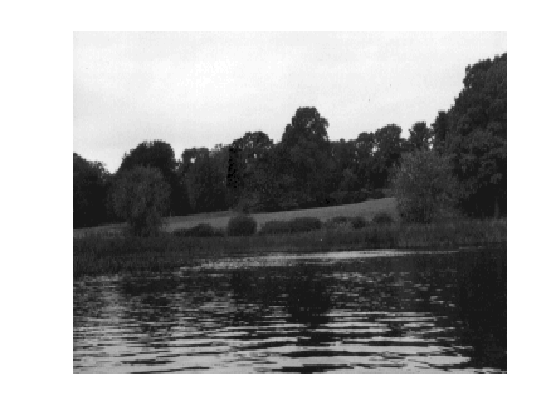
\includegraphics[width=\textwidth]{images/1/1-1-autumn_b.png}
% TODO 2/3 images
\end{figure}

\paragraph{Bords de l'image}
Le problème des bords de l'image est qu'ils ne repoussent pas pour l'instant le \emph{snake} or celui-ci ne devrait pas s'en approcher puisqu'on recherche les contours à l'intérieur de l'image. Pour résoudre ce problème il peut être pratique d'appliquer une force aux bords de l'image qui ramène le \emph{snake} vers l'intérieur de l'image.

\subsection{Exercice 2 - Implémentation du \emph{snake}}
\paragraph{Application à \emph{coins.png}}
Après implémentation de l'algorithme, on peut l'appliquer sur \emph{coins.png} et observer le résultat figure~\ref{7-coins}. Néanmoins les résultats varient beaucoup d'une pièce à l'autre car toutes n'ont pas le même contraste avec le fond.

\begin{figure}[!ht]
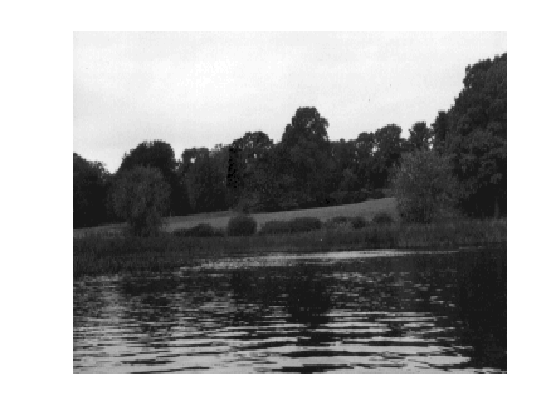
\includegraphics[width=\textwidth]{images/1/1-1-autumn_b.png}
% TODO 2/3 figures
\end{figure}

\paragraph{Application à \emph{IRM.png}}
De la même façon on peut appliquer l'algorithme pour détourer la tumeur sur \emph{IRM.png}; résultat figure~\ref{7-IRM}. On observe à nouveau une très forte variation de la qualité de l'algorithme selon comment est placé initialement le contour actif.

\begin{figure}[!ht]
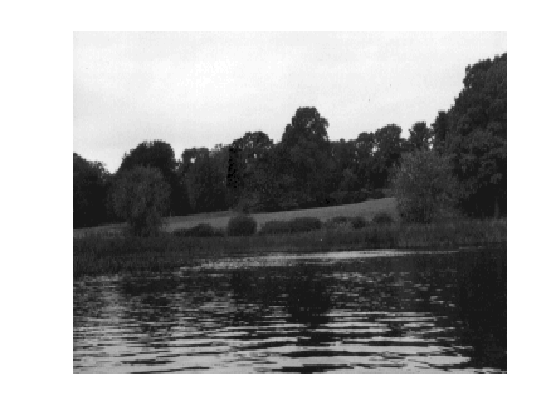
\includegraphics[width=\textwidth]{images/1/1-1-autumn_b.png}
% TODO 2/3 figures
\end{figure}

\subsection{Exercice 3 - Diffusion vers les contours}
\paragraph{Prolongement du champs de force}
Ici l'idée est de prolonger le champs de force là où il est faible par la valeur du champs de force élevé le plus proche. On crée donc une sorte de diagramme de voronoï avec le champs de force qui assurera que le \emph{snake} se déplace même si il est initialement mal placé. Près des bords le champs de force se comporte parfois étrangement et est très sujets aux petites perturbations. On peut observer ce nouveau champs de force et le résultat qu'il induit sur l'algorithme figure~\ref{7-diffusion}.

\begin{figure}[!ht]
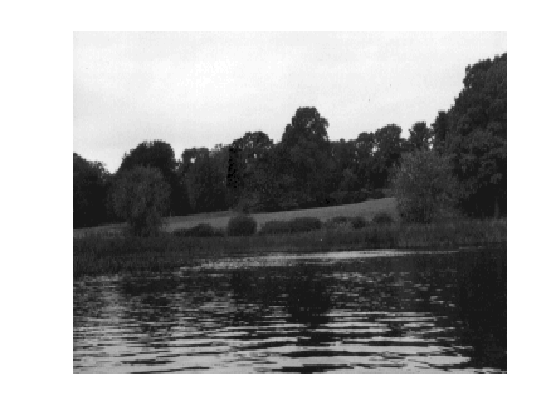
\includegraphics[width=\textwidth]{images/1/1-1-autumn_b.png}
% TODO 3/4 figures
\end{figure}

\paragraph{Inconvénients}
On observe que si les paramètres sont mal choisis le snake peut facilement se recroqueviller sur lui même. De plus les contours sont détectés très approximativement (à cause du flou gaussien). Enfin des snakes initiaux mals choisis peuvent faire se comporter étrangement l'algorithme qui va alors tenter de couvrir plusieurs contours simultanément.

\section{TP 8 - Restauration d'images}
On a déjà dans un TP précédent étudier une méthode de restauration d'image qui consistait à projeter les parties préservées dans une base connue pour considérer alors la projection comme image restaurée. Cette fois ci on s'intéresse à un mécanisme indépendant d'une base préalable et capable de remplacer les zones altérées d'une image à partir de la connaissance du reste de l'image uniquement.

\subsection{Exercice 1 - Tikhonov}
\paragraph{Modélisation variationelle}
Dans un premier temps on s'intéresse à la restauration d'une image bruitée. Pour cela on va utiliser une approche variationelle après modélisation du problème. La proximité de l'image originale avec l'image restauré ainsi que le caractère "lisse" de celle restaurée conduit à l'établissement de l'énergie dite de Tikhonov présentée dans le sujet. La minimiser dans le cas d'une image numérique conduit à la résolution de l'équation d'Euler-Lagrange discrète :
\[\lambda [I_N - (-D_x^TD_x - D_y^TD_y)]u = \lambda u_0\]

\paragraph{Influence de $\lambda$}
Après implémentation on observe les résultats figure~\ref{8-tikhonov}.

\begin{figure}[!ht]
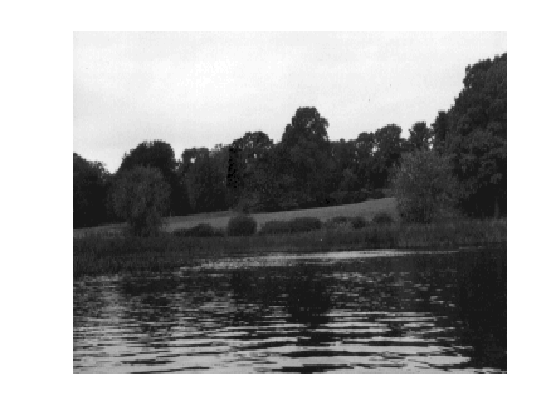
\includegraphics[width=\textwidth]{images/1/1-1-autumn_b.png}
% TODO 3/4 figures
\end{figure}

On remarque que plus $\lambda$ est petit, plus le bruit disparait mais plus les contours sont floutés; cela n'est pas étonnant à la vue de l'équation variationelle qui rend alors prédominant le terme dû au gradient de l'image (qui est alors minimisé ce qui floute l'image).

\subsection{Exercice 2 - Débruitage par variation totale}
\paragraph{Variation totale}
Pour palier le problème des contours que la minimisation de l'équation de Tikhonov tend à faire disparaître on décide de remplacer le carré de la norme du gradient par la norme du gradient. La norme n'étant pas différentiable on choisit de la remplacer par une fonctione approximante qui est différentiable puis on résoud l'équation variationelle induite. On observe alors les résultats figure~\ref{8-variation-totale}.

\begin{figure}[!ht]
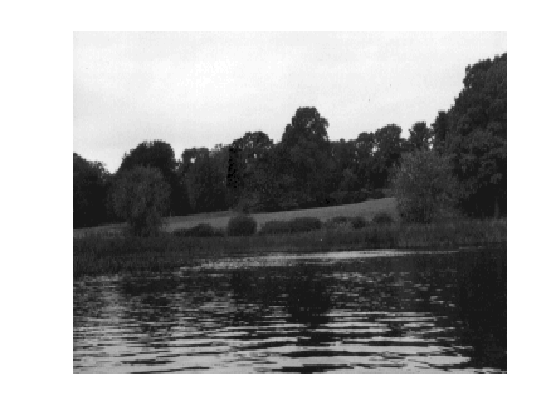
\includegraphics[width=\textwidth]{images/1/1-1-autumn_b.png}
% TODO 2/3 images
\end{figure}

\paragraph{Image RVB}
Dans le cas des images RVG l'algorithme peut être appliqué à chaque canal séparément pour obtenir une image moins bruitée. En l'appliquant sur \emph{lena.bmp} on obtient le résultat de la figure~\ref{8-lena}.

\begin{figure}[!ht]
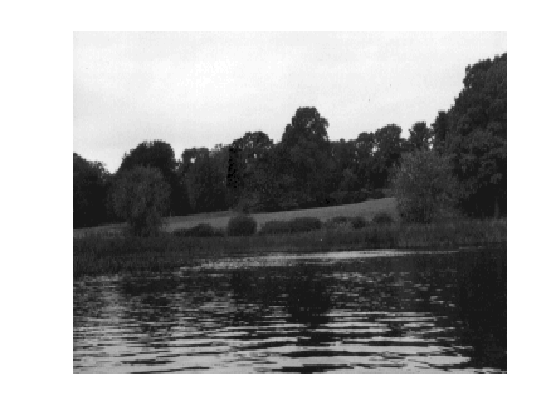
\includegraphics[width=\textwidth]{images/1/1-1-autumn_b.png}
% TODO 2/3 images
\end{figure}

\subsection{Exercice 3 - Inpainting}
\paragraph{Équation variationelle}
L'inpainting consiste à remplacer une partie d'une image par une texture calculée à partir de ce qui entoure cette partie. On peut là encore modéliser ce problème sous la forme d'une équation variationelle que présente et résoud le sujet. On obtient des résultats très concluants lorsque l'on dispose du masque à enlever (figure~\ref{8-inpainting}).

\begin{figure}[!ht]
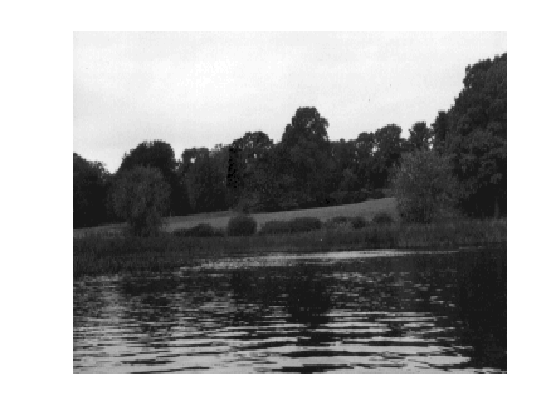
\includegraphics[width=\textwidth]{images/1/1-1-autumn_b.png}
% TODO 2/3 images
\end{figure}

\paragraph{Calcul du masque}
Dans le cas où l'on ne dispose pas au préalable du masque à remplacer on peut calculer celui-ci par exemple en effectuant un seuillage de l'image. Cela fonctionne très bien pour l'image \emph{grenouille.png} figure~\ref{8-grenouille}.


\section{TP 9 - Retouche d'images}
Dans la lignée des TPs précédents, celui-ci montre comment les équations variationelles peuvent être utilisée pour faire de la retouche d'image consistant en le remplacement d'une partie d'une image par une autre image.

\subsection{Introduction}
La solution naïve consiste à simplement placer la nouvelle image à la place de la partie à remplacer (figure~\ref{9-naive}). Cependant comme on peut le voir cela ne rend pas du tout bien : d'une part la chromatographie n'est pas respectée de l'image originale à l'image remplaçante, d'autre part le gradient à l'endroit de la jonction est très élevé donc irréaliste.

\begin{figure}[!ht]
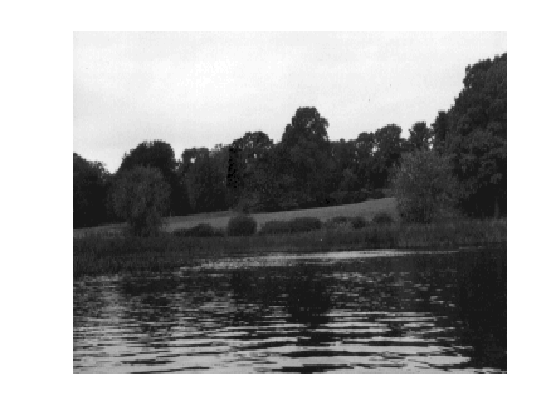
\includegraphics[width=\textwidth]{images/1/1-1-autumn_b.png}
% TODO 1 image
\end{figure}

\subsection{Exercice 1 - Condition de Neumann}
L'implémentation de l'algorithme donné par le sujet donne le résultat figure~\ref{9-neumann}. Afin de palier le fait que le rang de A ne soit pas maximal, j'ai choisis d'appliquer la contrainte qui impose de conserver la moyenne de la couleur sur le bord de la zone à remplacer.

\begin{figure}[!ht]
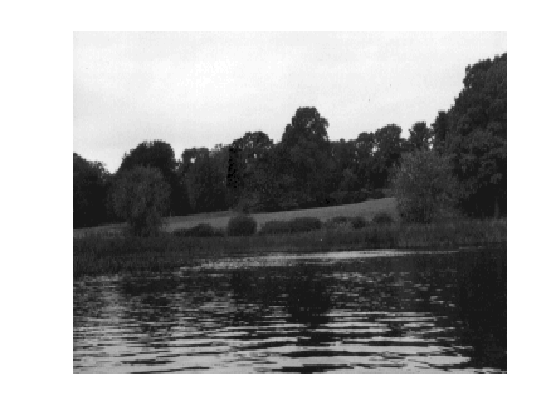
\includegraphics[width=\textwidth]{images/1/1-1-autumn_b.png}
% TODO 1 image
\end{figure}

Le résultat est cette fois-ci bien meilleur puisque la chromatographie semble la même sur les deux parties de la nouvelle image. Cependant il y a encore le problème de la jonction entre ces deux parties qui n'a pas été traité. La raison est que l'équation variationelle tient ne tient compte que de la zone à remplacer et non de sa jonction avec le reste de l'image.

\subsection{Exercice 2 - Condition de Dirichlet}
La condition de Dirichlet permet de résoudre le problème ennoncé plus haut en imposant une condition sur le bord de l'imagette à coller. Après implémentation on obtient un résultat presque impécable (figure~\ref{9-dirichlet}).


\section{TP 10 - Décomposition \emph{cartoon}+texture d'une image}
Ce TP présente les différentes façon d'opérer sur une image une décomposition cartoon+texture.

\subsection{Exercice 1 - Partition du spectre d'une image}
Dans le premier exercice on opère simplement une décomposition entre les hautes et les basses fréquences, la fréquence de coupure étant choisie arbitrairement en fonction de l'image. En effet la fréquence des textures dépend fortement de l'image, de sa taille et du type d'informations qu'elle contient; dans tous les cas les fréquences hautes représentent la partie texture tandis que les fréquences basses représentent la partie \emph{cartoon} (figure~\ref{10-decomposition}). Dans ce cas la fréquence de coupure retenue est de 32.

\begin{figure}[!ht]
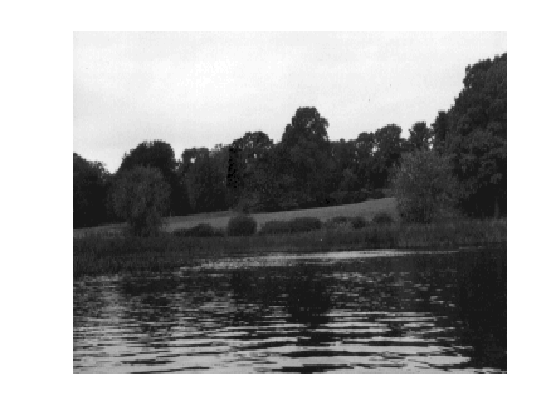
\includegraphics[width=\textwidth]{images/1/1-1-autumn_b.png}
% TODO 6 images
\end{figure}

On remarque qu'on ne pas a obtenir de résultat convainquant car dans certaines parties de l'image la texture est de fréquence plus haute que dans d'autres, d'où l'impossibilité de choisir une valeur adéquate pour la fréquence de coupure qui ne fasse pas retenir trop ou pas assez de fréquences pour la texture (et inversement pour le \emph{cartoon}) dans certaines parties de l'image.

\subsection{Exercice 2 - Filtrage spectral}
Afin de palier le problème ennoncé plus haut on décide alors non pas de choisir une fréquence de coupure mais de lisser la séparation entre les fréquences de la partie \emph{cartoon} et celles de la partie texture. On obtient les résultats de la figure~\ref{10-filtrage} qui sont plus convainquants.

\begin{figure}[!ht]
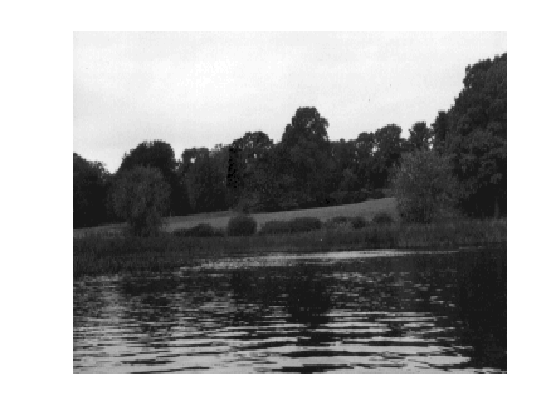
\includegraphics[width=\textwidth]{images/1/1-1-autumn_b.png}
% TODO 6 images
\end{figure}

\subsection{Exercice 3 - Modèle ROF}
Une fois n'est pas coutûme on peut modéliser le problème de séparation des hautes et basses fréquences par une équation variationelle. En appliquant l'algorithme itératif suggéré par l'ennoncé à l'image de l'actrice on obtient un résultat encore meilleur que celui de l'exercice précédent. Cependant c'est bien sur l'image \emph{empreinte.png} que cela est le plus spéctaculaire puisqu'elle paraît parfaitement "reconnue" par l'algorithme tandis qu'un seuillage ne réussi pas du tout cette tâche (figure~\ref{10-empreinte}).

\begin{figure}[!ht]
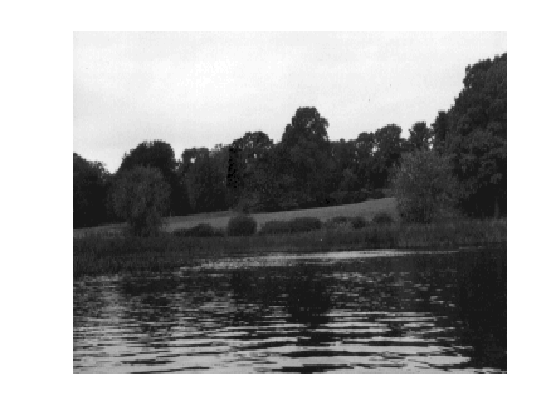
\includegraphics[width=\textwidth]{images/1/1-1-autumn_b.png}
% TODO n images
\end{figure}

Cela est certainement dû au fait que la résolution de l'équation variationelle du modèle ROF permet de prendre en compte en chaque point de l'image une analyse de son environnement local pour le traiter au mieux.

\subsection{Exercice 4 - Modèle TV-Hilbert}
Dans cette dernière partie on applique un modèle variationelle qui diffère encore puisqu'il fait intervenir la transformée du Fourier du signal à retrouver (l'image \emph{cartoon}). La pronfonde non linéarité de la transformation de Fourier empèche une résolution aussi directe que précédement : on doit donc mettre en place une descente de gradient pour résoudre ce problème. Après résolution on obtient pour l'empreinte les résultats de la figure~\ref{10-hilbert}.

\begin{figure}[!ht]
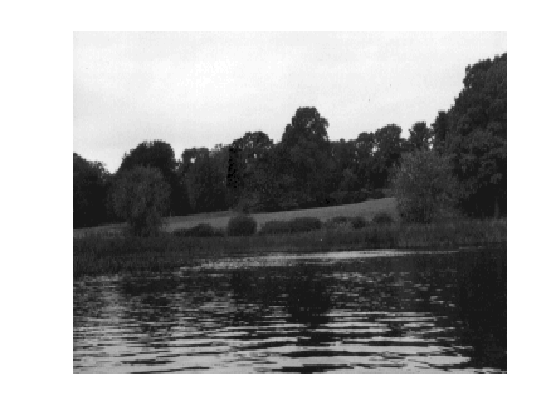
\includegraphics[width=\textwidth]{images/1/1-1-autumn_b.png}
% TODO n images
\end{figure}




\section{TP 11 - Transformation de Gabor}
On s'intéresse dans ce TP à différents cas d'utilisation pratiques de la transformée de Gabor qui permet de représenter sous la forme d'une image une empreinte accoustique d'un enregistrement audio.

\subsection{Exercice 1 - Transformée de Gabor}
\paragraph{La transformée de Gabor et son inverse}
Dans un premier temps on effectue la transformée de Gabor avec une fenêtre glissante dont l'image partitionne le temps d'enregistrement. On peut alors retrouver l'enregistrement initial à partir de la transformée de Gabor (figure~\ref{11-gabor}). On remarque que cela n'est pas possible avec la porteuse Gaussienne qu'utilisait Gabor à la place de la fenêtre glissante.

\begin{figure}[!ht]
\includegraphics[width=\textwidth]{images/1/1-1-autumn_b.png}
% TODO 3 images
\end{figure}

\paragraph{Altération}
On se propose de ne conserver que la partie réelle de la transformée de Gabor puis que le module, et d'effectuer pour ces deux cas la transformée de Gabor inverse. On observe alors que TODO

\subsection{Exercice 2 - Sonagramme}
\paragraph{Restriction des fréquences}
Cette fois ci on retire les fréquences négatives et les fréquences trop grandes. Le signal se dégrade assez rapidement lorsqu'on retire les hautes fréquences (figure~\ref{11-sonagramme} puisqu'il suffit de TODO pourcents pour entendre la différence. On a alors retiré au total TODO pourcents des fréquences : ce n'est pas si mal.

\paragraph{Altération}
Cette fois ci TODO(module/partie réelle)

\subsection{Exercice 3 - Création de la partition à partir du sonagramme}
Désormais on va compresser encore la représentation du sonagramme en le mettant sous la forme d'une partition. Pour cela on détermine pour chaque mesure la fréquence la plus importante et c'est celle qui correspondra à la note sur la partition (ce n'est en réalité pas exact car une note sur un instrument produit généralement plusieurs fréquences simultanément et parfois la plus audible n'est pas celle attendue). Après implémentation de l'algorithme, le résultat obtenu est celui présenté figure~\ref{11-partition}.

\begin{figure}[!ht]
\includegraphics[width=\textwidth]{images/1/1-1-autumn_b.png}
% TODO 1/2 images
\end{figure}

\subsection{Exercice 4 - Compression audio}
Le but est d'utiliser la représentation sous la forme de partition comme enregistrement audio compressé. On peut alors à partir de celle-ci retrouver le sonagramme puis par transformation de Gabor inverse obtenir le son. Comme en conservant une note par mesure on perd trop d'informations, on décide de retenir pour chaque mesure un nombre n de notes (fréquences), à condition que leur coefficient dépasse un certain seuil.

TODO


\section{TP 12 - Shazam}
Ce TP nous fait étudier, dans la continuité du précédent, un cas
d'utilisation de l'empreinte sonore que nous avons réalisé. Il s'agit
de la reconnaissance de morceau telle qu'effectuée par Shazam.

\subsection{Exercice 1 - Empreinte sonore}
Dans le TP précédent nous avons effectué une empreinte sonore sur tout le
morceau en conservant mesure par mesure la fréquence la plus importante.
Cette fois ci on décide de découper l'intervalle de fréquence en 6 bandes
(environ 1.5 octaves) puis de sélectionner dans chacune et pour chaque
mesure la fréquence la plus importante : cela constitue l'empreinte de
l'enregistrement sonore. Pour le son \emph{007.wav} on obtient le
rélsutat figure~\ref{12-007}.

\begin{figure}
% TODO 1 image
\end{figure}

\subsection{Exercice 2 - Comparaison d'empreintes}
Pour cette exercice on doit calculer un score de ressemblance d'un
enregistrement à une partie d'un autre. A ces fins on calcule une
certaine distance du sonagramme du premier à celui du second.

\paragraph{Distance euclidienne}
D'après les indications du sujet (et les informations récoltées a
posteriori auprès des enseignants) il semblerait que la distance
attendue soit une distance euclidienne. Cependant cela ne m'apparaît
pas du tout judicieux car fréquences et temps ne sont pas de même
"type" ni de même ordre de grandeur. De plus comme il s'agit de
morceaux de musique, la fréquence augmente exponentiellement (on
pourrait donc prendre le logarithme de la fréquence ce qui serait déjà
plus juste). Le résultat de la fistance euclidienne la plus simple est
visible figure~\ref{12-euclidienne}.

\begin{figure}
% TODO 2 images
\end{figure}

\paragraph{La mesure}
N'ayant pas pu assister à la séance pour ce TP j'ai bloqué pendant
plusieurs heures chez moi à cause de la variable \emph{mesure} présente
dans le code de cet exercice. En effet bien que ce terme n'ait pas de
signification précise en musique, il est souvent employé pour définir
un ensemble de plusieurs notes qui dure généralement un temps comparable
à la seconde. J'ai donc longtemps bloqué sur ce dernier car je cherchait
à établir une distance convenable mais m'appercevait que celle-ci était
parfois de plusieurs mesures ! (voir ci dessous). Puis j'ai remarqué
que la valeur d'une mesure était très faible et ne représentait
certainement pas la mesure usuelle en musique mais plutôt le pas
"d'échantillonage" du sonagramme.

\paragraph{Distance sensée}
Afin de choisir une distance qui ait une réelle signification j'ai
préféré réfléchir de manière pratique : tout d'abord si une fréquence est
dans l'extrait elle devra se retrouver dans les données avec une valeur
très proche (de moins que la différence entre deux notes successives
vraisemblablement). En comparant les logarithme en base 10 de deux notes
ceux ci ne doivent donc pas dépasser \emph{log10(1+1/15)}, 15 étant le
nombre de demi tons sur une octave. Ainsi une fois trouvée dans les données
la note avec la même fréquence à cet écart près, on peut comparer la
distance en temps qui est celle que l'on retient. J'obtient alors des
résultats qui me paraissent bien plus "sensés" (figure~\ref{12-distance}).

\begin{figure}
% TODO 1 figure
\end{figure}

\subsection{Exercice 3 - Shazam}
Dans cette dernière partie on tire profit de la distance créée précédement
pour comparer un extrait à plusieurs morceaux afin de déterminer duquel
il provient. On obtient des résoultats très concluants (ça fonctionne à
chaque fois pour les extraits fournis).

\paragraph{Améliorations}
Bien que cet algorithme soit celui utilisé par le leader du marché, il y a
fort à parier qu'il n'est pas le plus efficace puisque l'un de ses
concurents (soundhound) parvient même à reconaître une musique
sifflotée (notre algorithme ne pourraît comparer correctement un tel
extrait puisqu'il est très rare qu'on siffle "juste", c'est à dire avec
la même fréquence).

\section{TP 13}
\section{TP 14}

\end{document}
